\section{Impact of Resoved Signal Region Veto }
\label{app:resveto}

\paragraph{}
To further check the impact of vetoing 4$b$ tagged events with resolved signal region $Xhh < 1.6$ cut, we loose the cut to $Xhh < 3.2$ and test the resolved veto again. For $4b$ boosted background estimation, the $2b$ events are also required to exclude events with $Xhh < 3.2$ and at least two resovled $b$ tagged jets. Another test is to fully veto every event with at least four $b$ tagged AntiKT4 jets. In this case, the 4b \ttbar MC runs out of statistics in the Sideband region. Figure ~\ref{fig:app-resveto-sb} shows the distribution before any reweighting, for $4/3/2b$s in the Sideband region, with the resolved Signal region veto, loose Signal region veto, and full veto; and Figure ~\ref{fig:app-resveto-cr} shows the corresponding Control region.

\paragraph{}
Overall, the impact on the Sideband and Control region is small for 2$b$s and 3$b$. For 4$b$, some changes in the Sideband region yield is observed, yet the modeling in the Sideband and Control region appears to be fairly good. 

\begin{figure*}[htbp!]
\begin{center}
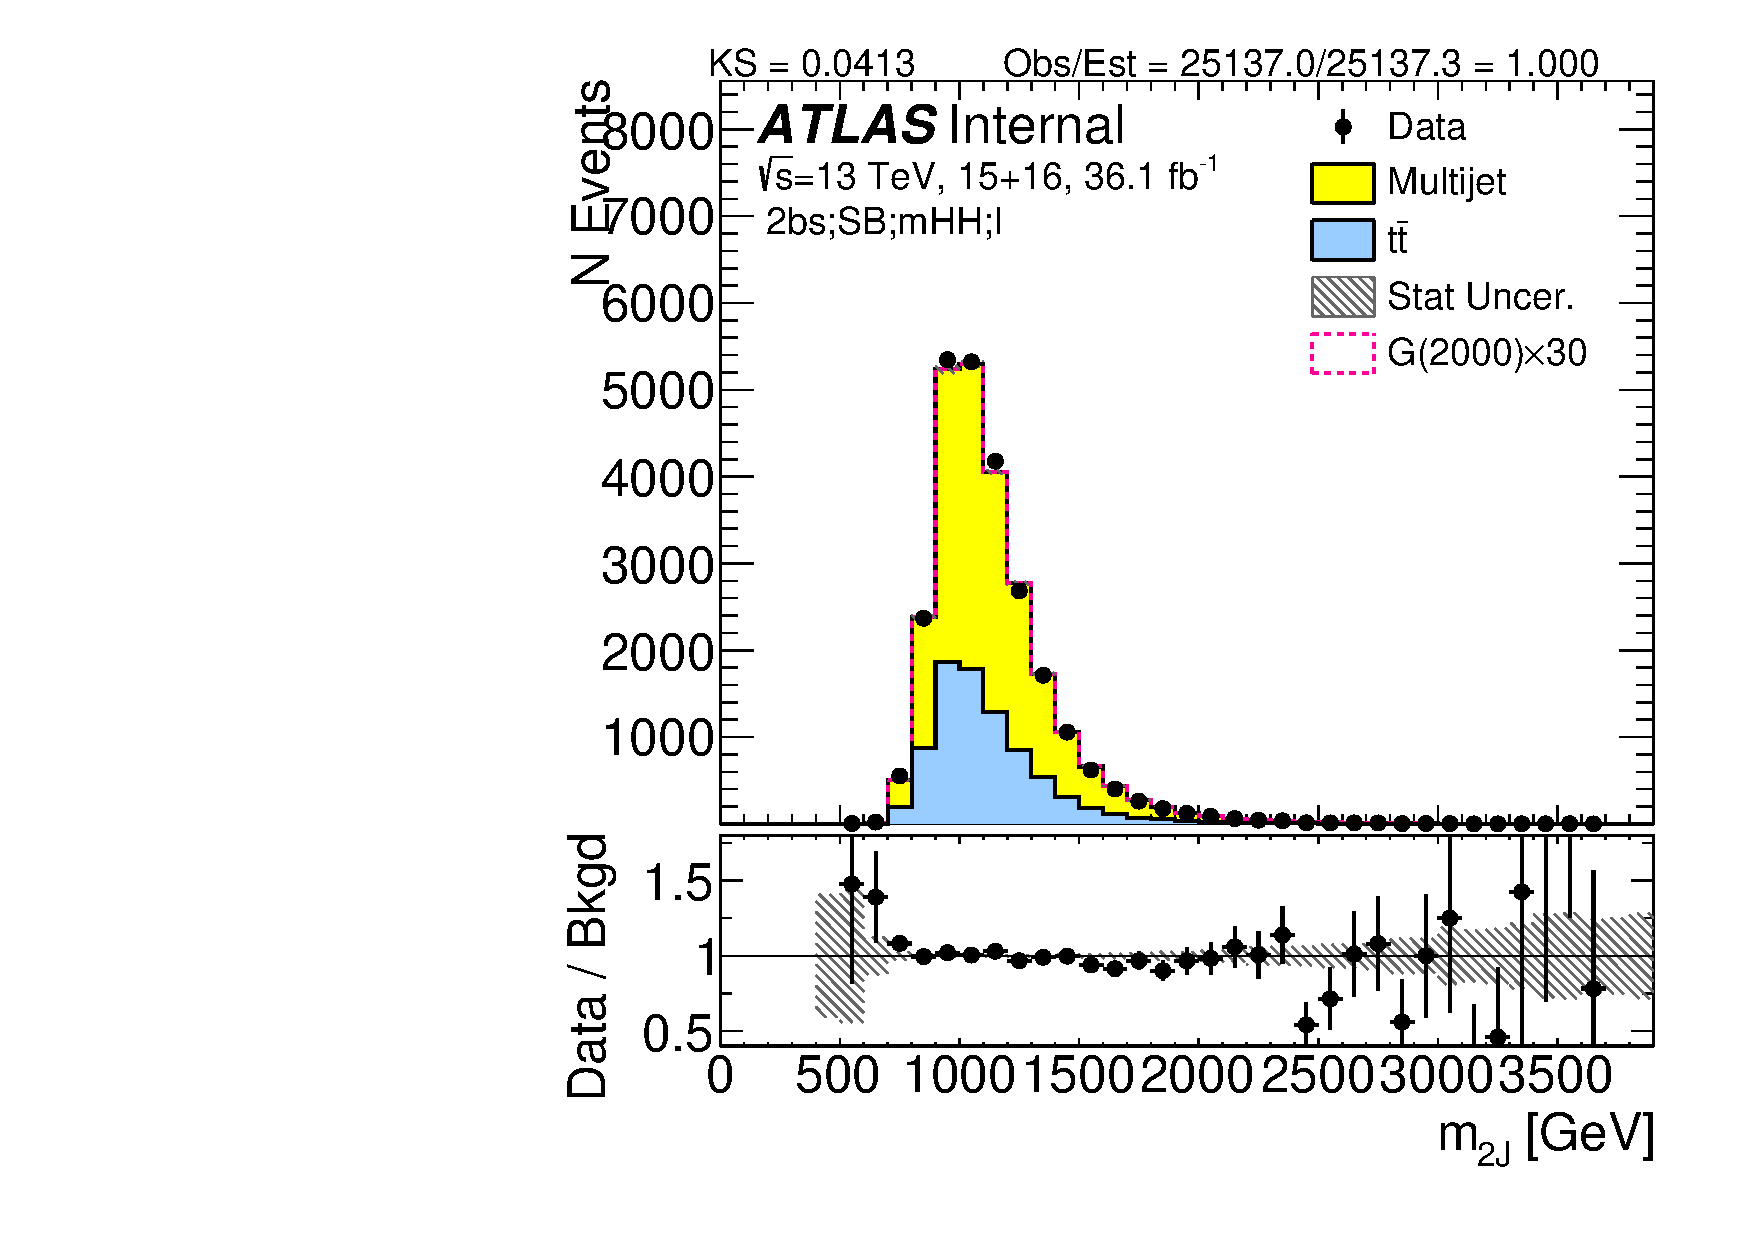
\includegraphics[angle=270, width=0.3\textwidth]{./figures/boosted/AppendixResveto/Moriond_TwoTag_split_Sideband_mHH_l.pdf}
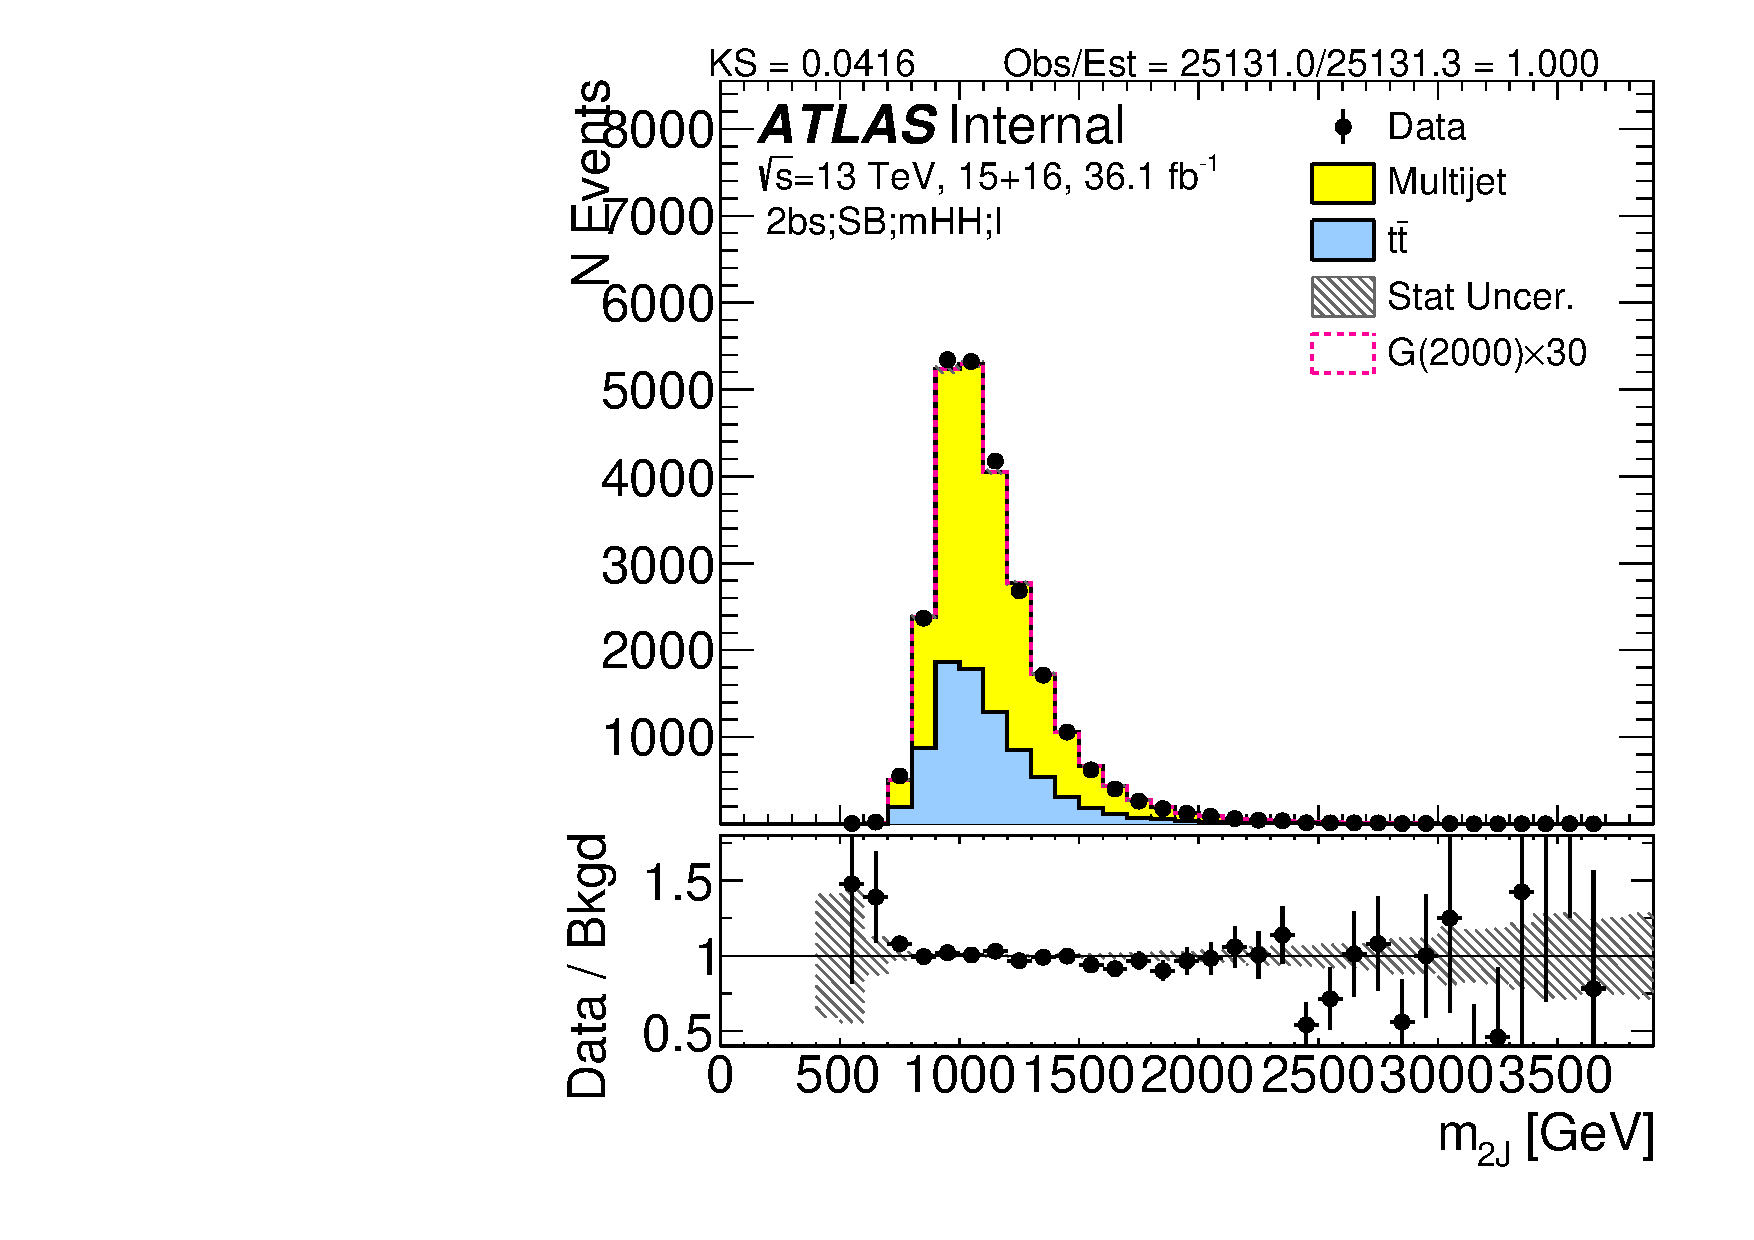
\includegraphics[angle=270, width=0.3\textwidth]{./figures/boosted/AppendixResveto/Moriond_resveto_TwoTag_split_Sideband_mHH_l.pdf}
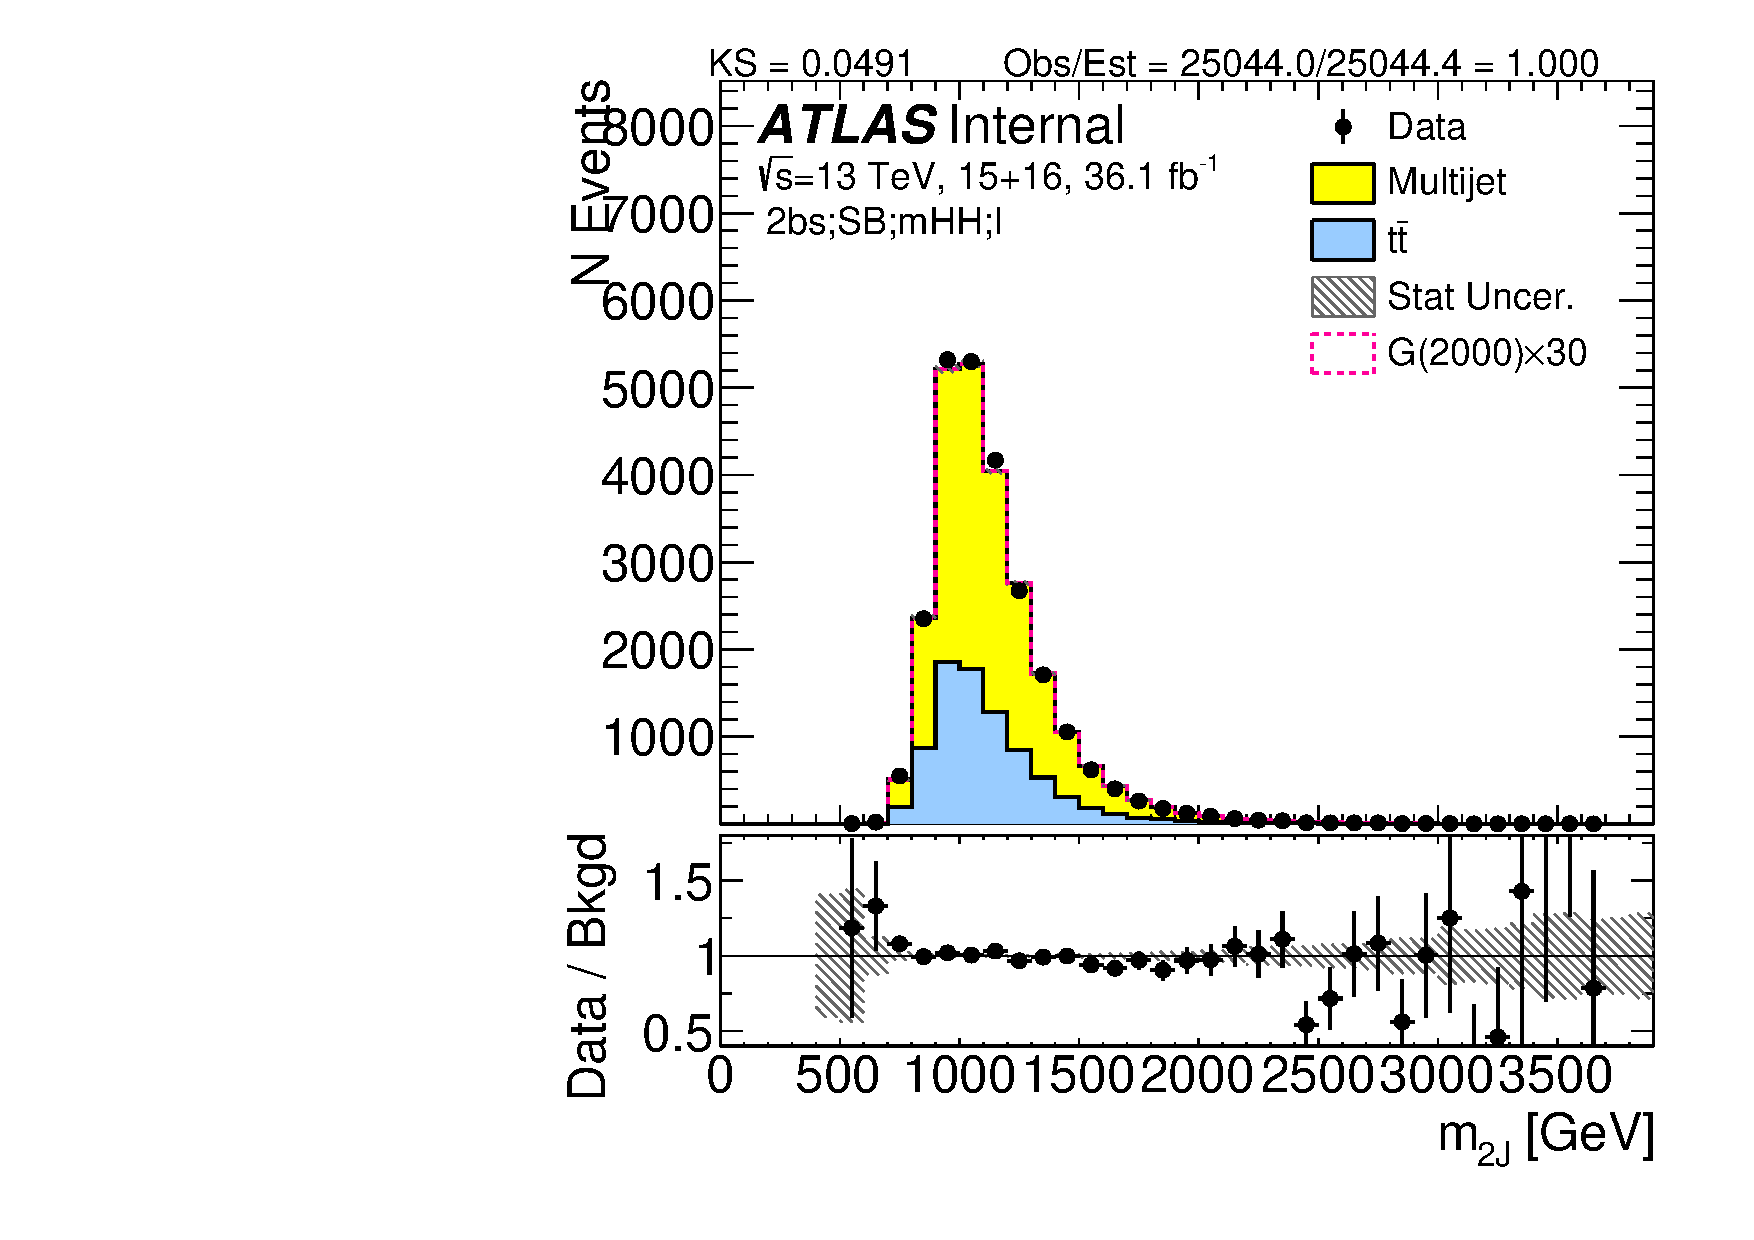
\includegraphics[angle=270, width=0.3\textwidth]{./figures/boosted/AppendixResveto/Moriond_fullresveto_TwoTag_split_Sideband_mHH_l.pdf}\\
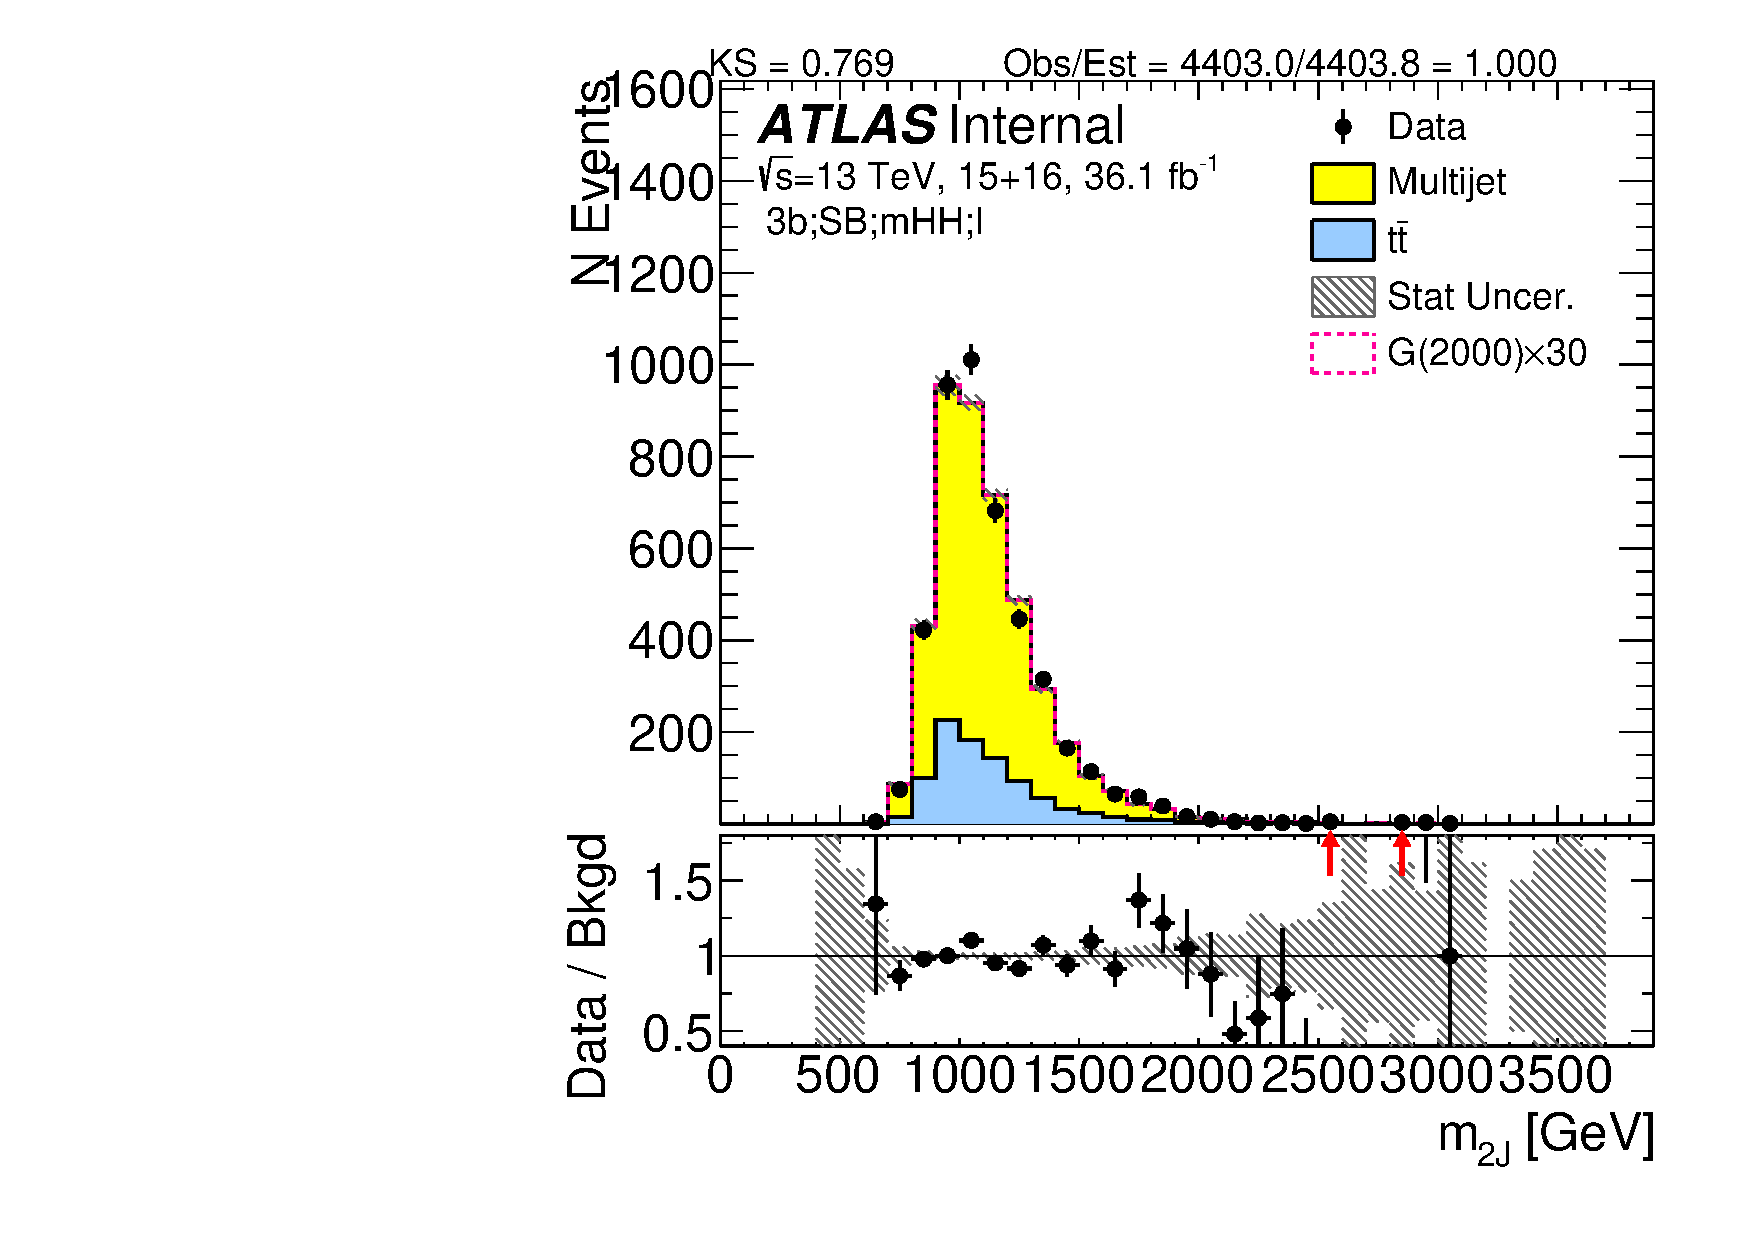
\includegraphics[angle=270, width=0.3\textwidth]{./figures/boosted/AppendixResveto/Moriond_ThreeTag_Sideband_mHH_l.pdf}
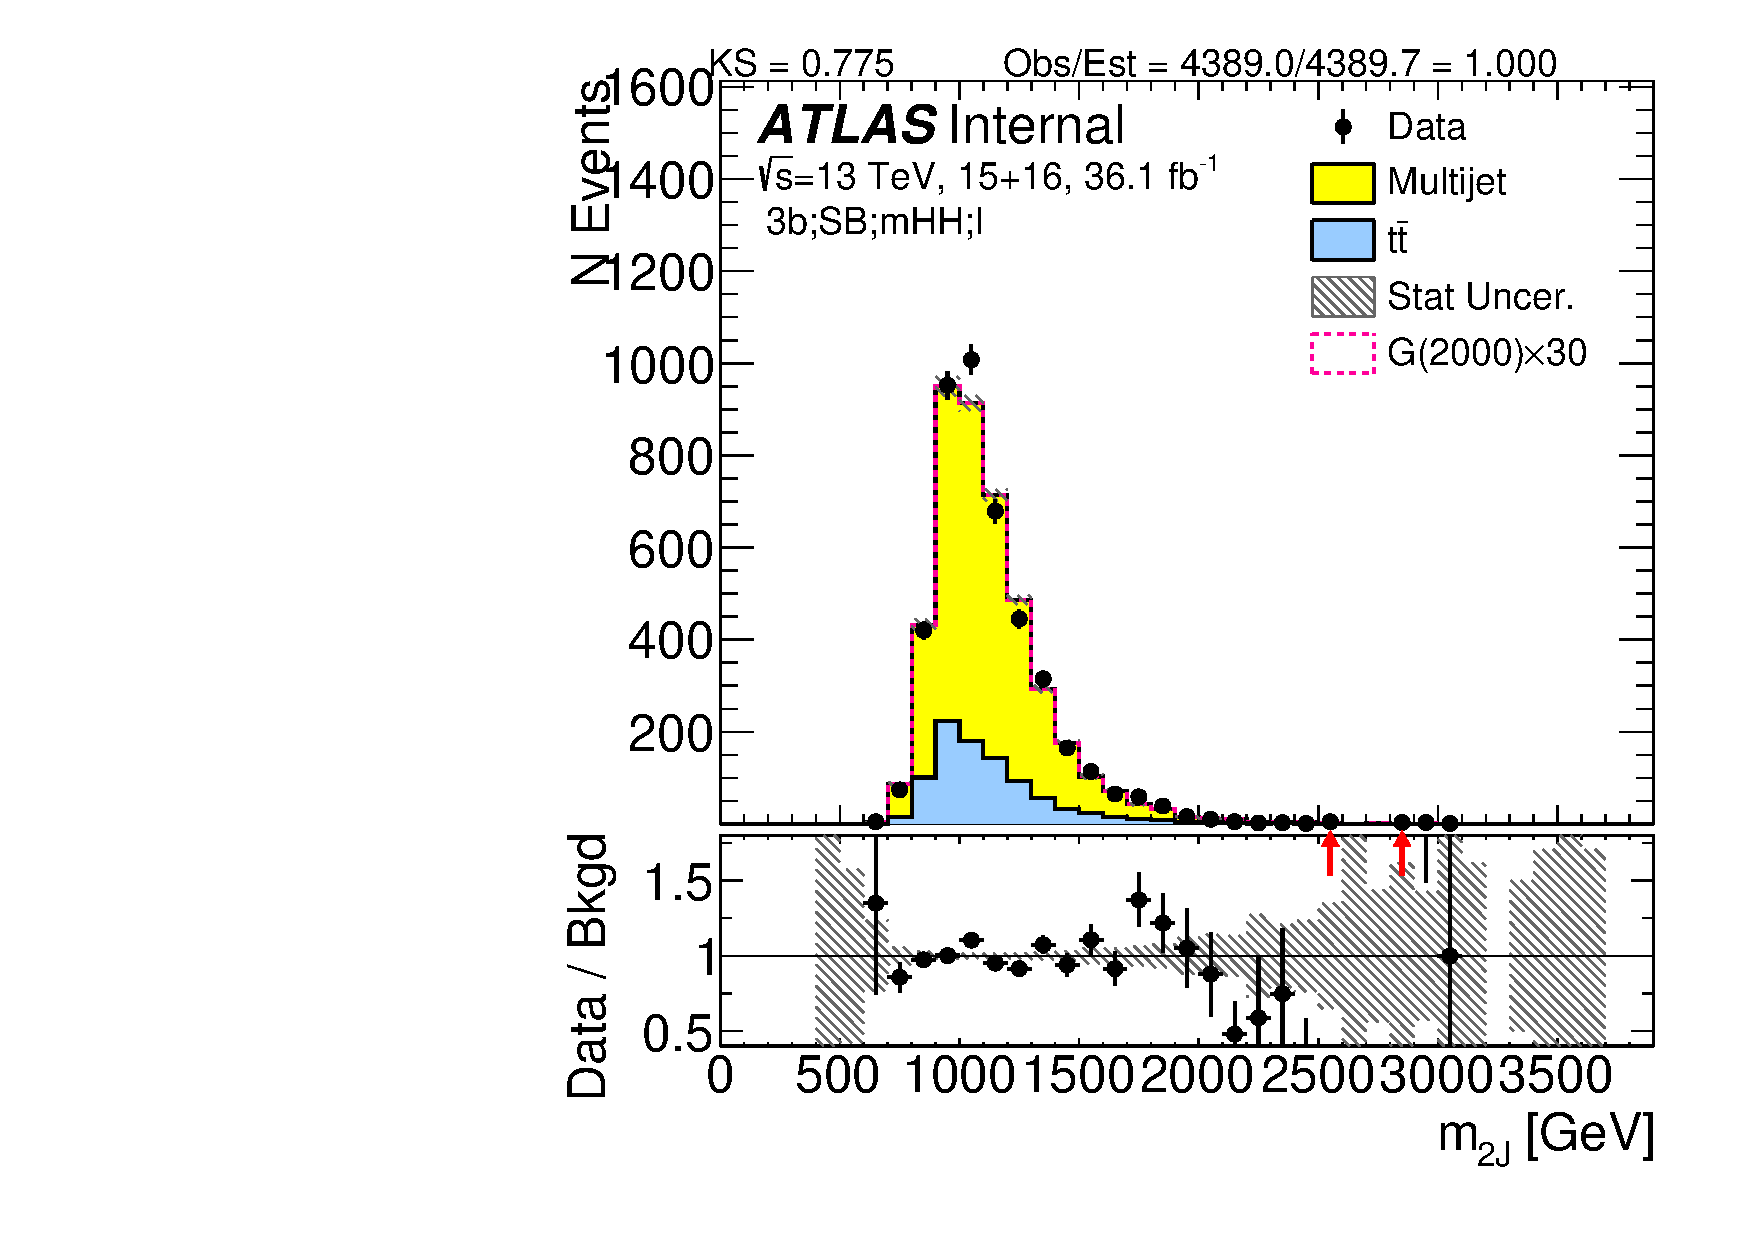
\includegraphics[angle=270, width=0.3\textwidth]{./figures/boosted/AppendixResveto/Moriond_resveto_ThreeTag_Sideband_mHH_l.pdf}
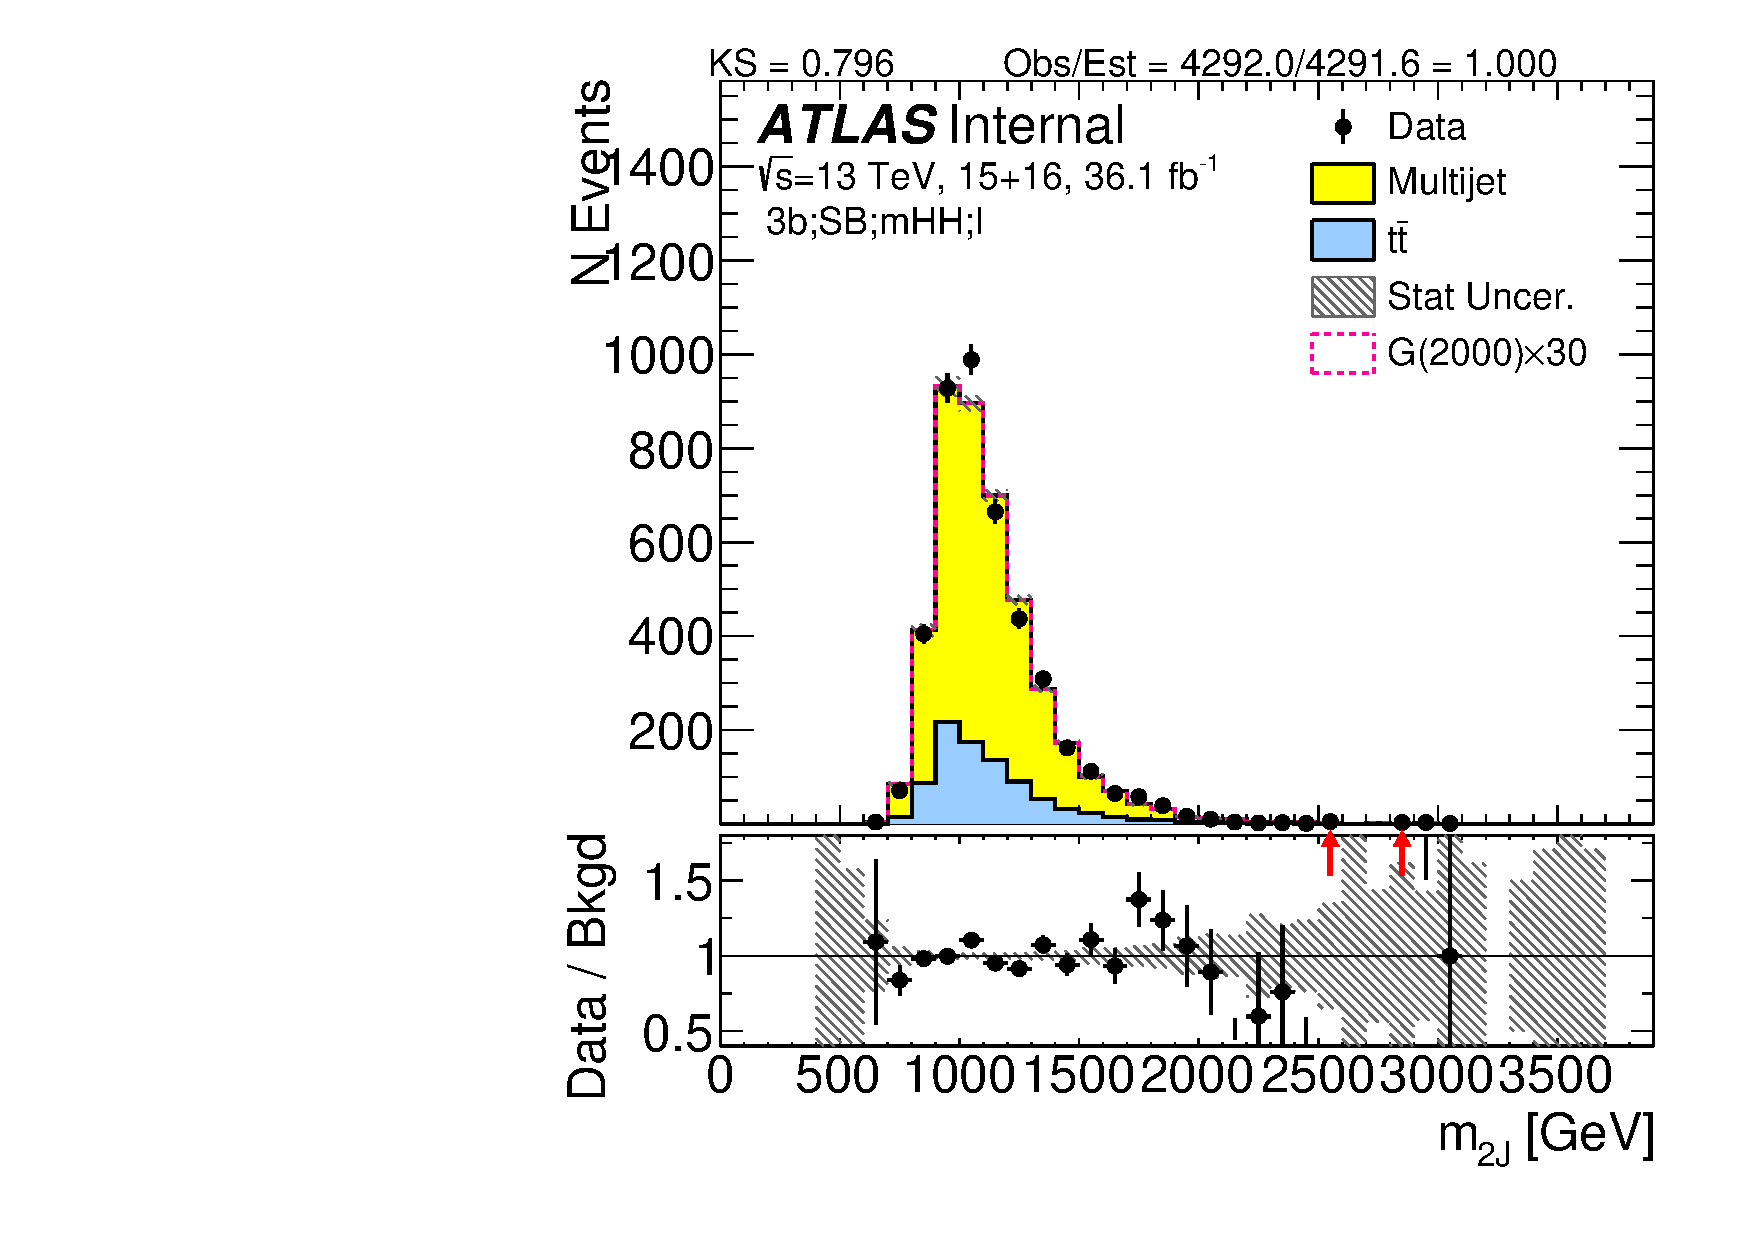
\includegraphics[angle=270, width=0.3\textwidth]{./figures/boosted/AppendixResveto/Moriond_fullresveto_ThreeTag_Sideband_mHH_l.pdf}\\
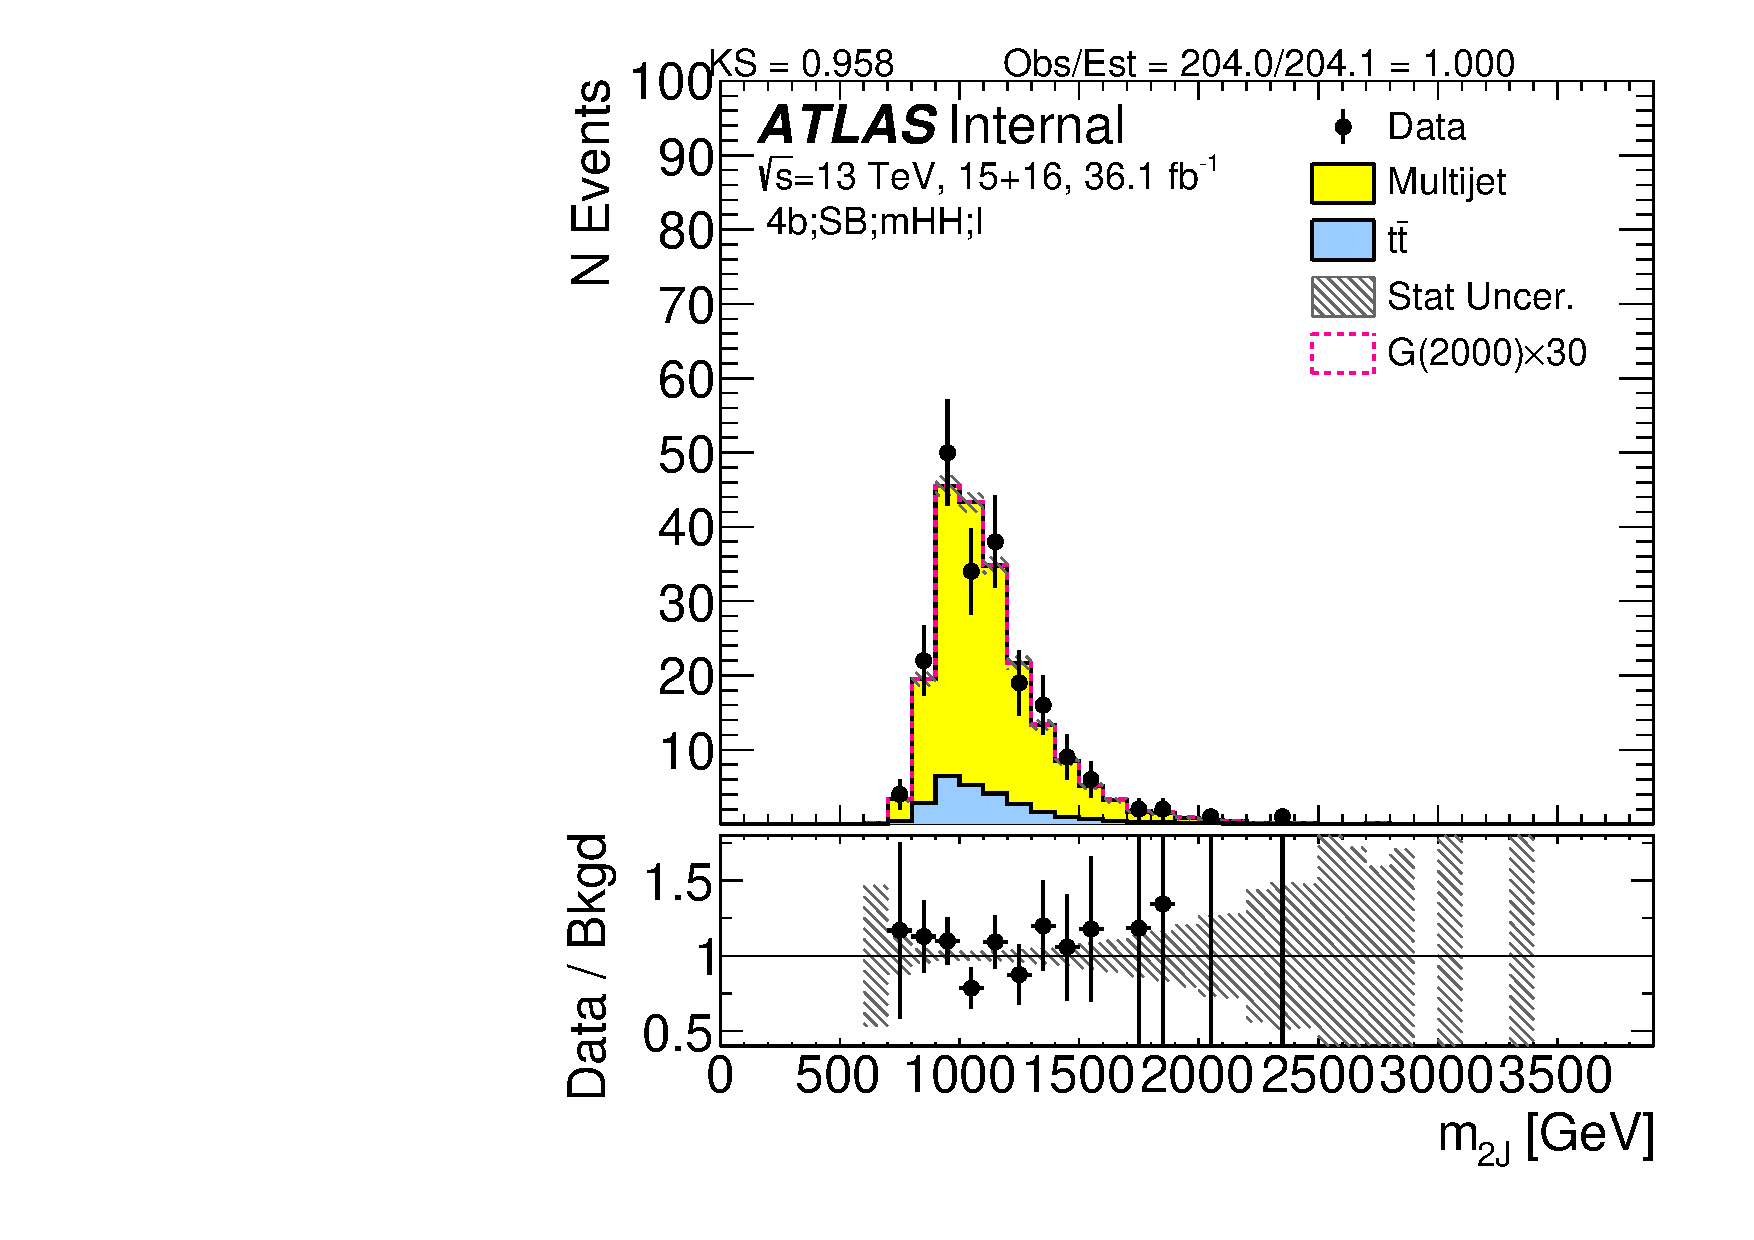
\includegraphics[angle=270, width=0.3\textwidth]{./figures/boosted/AppendixResveto/Moriond_FourTag_Sideband_mHH_l.pdf}
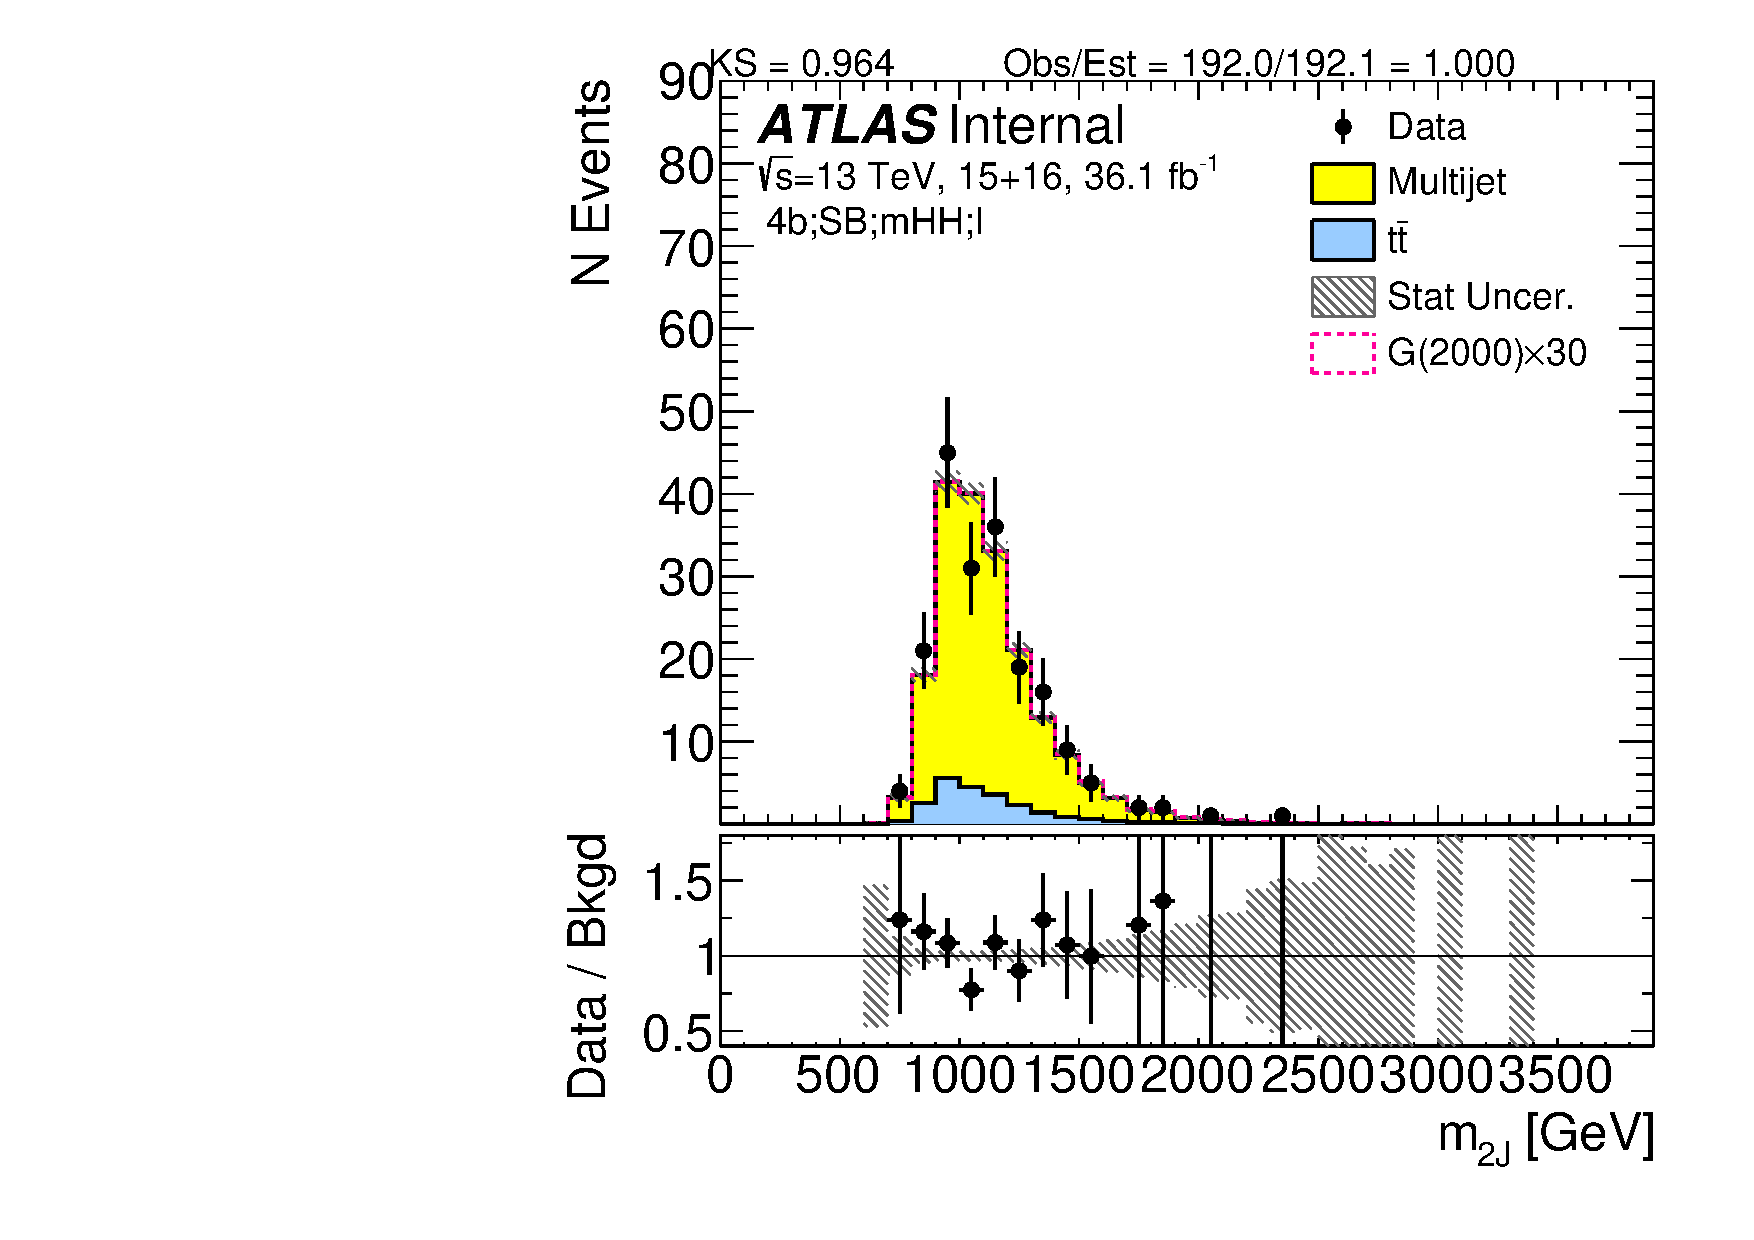
\includegraphics[angle=270, width=0.3\textwidth]{./figures/boosted/AppendixResveto/Moriond_resveto_FourTag_Sideband_mHH_l.pdf}
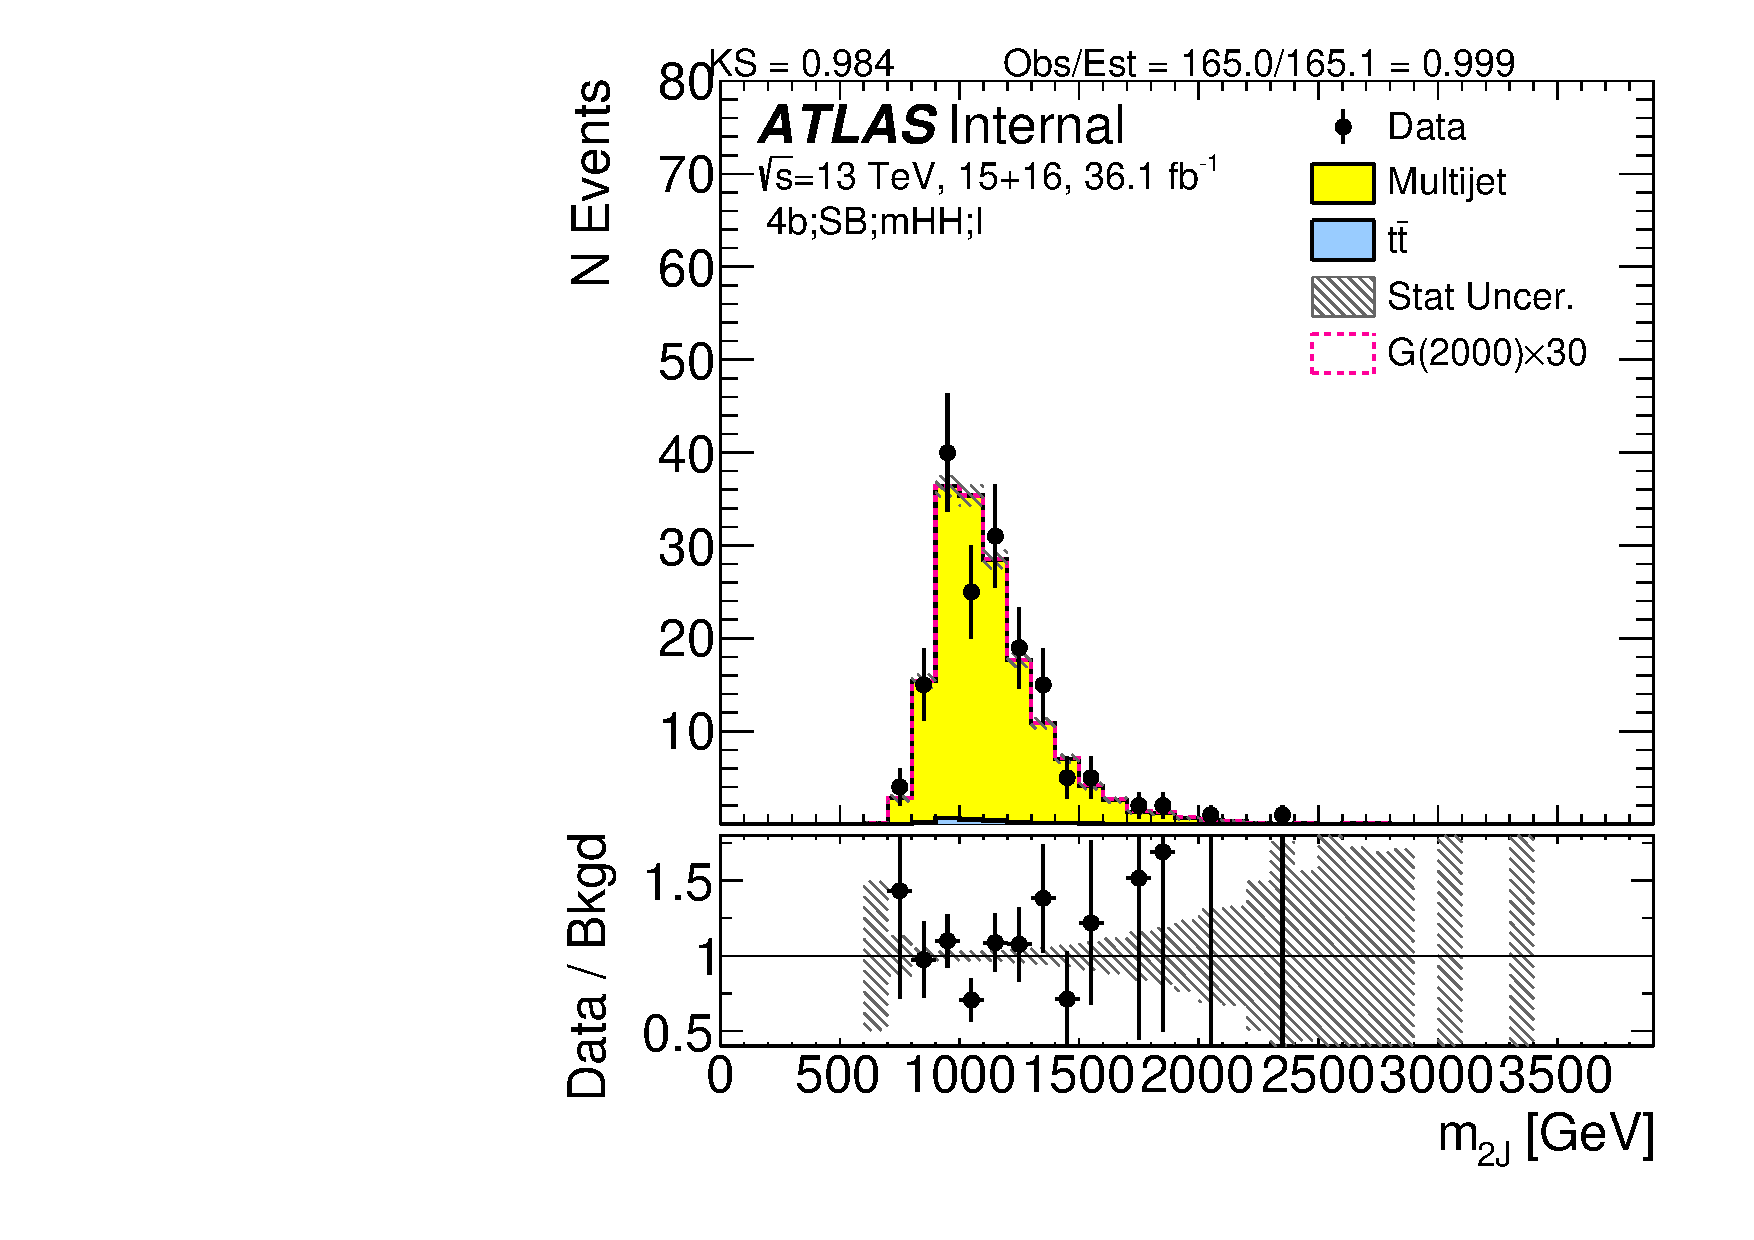
\includegraphics[angle=270, width=0.3\textwidth]{./figures/boosted/AppendixResveto/Moriond_fullresveto_FourTag_Sideband_mHH_l.pdf}\\
  \caption{ $M_{JJ}$ distribution in Sideband region for 2$b$s(top), 3$b$ (middle) and 4$b$ (bottom). The left column is with the stanard resovled veto; the middle column is with the loose resolved Signal Region, $Xhh < 3.2$ veto; the right column is with the full resolved veto.}
\label{fig:app-resveto-sb}
\end{center}
\end{figure*}

\begin{figure*}[htbp!]
\begin{center}
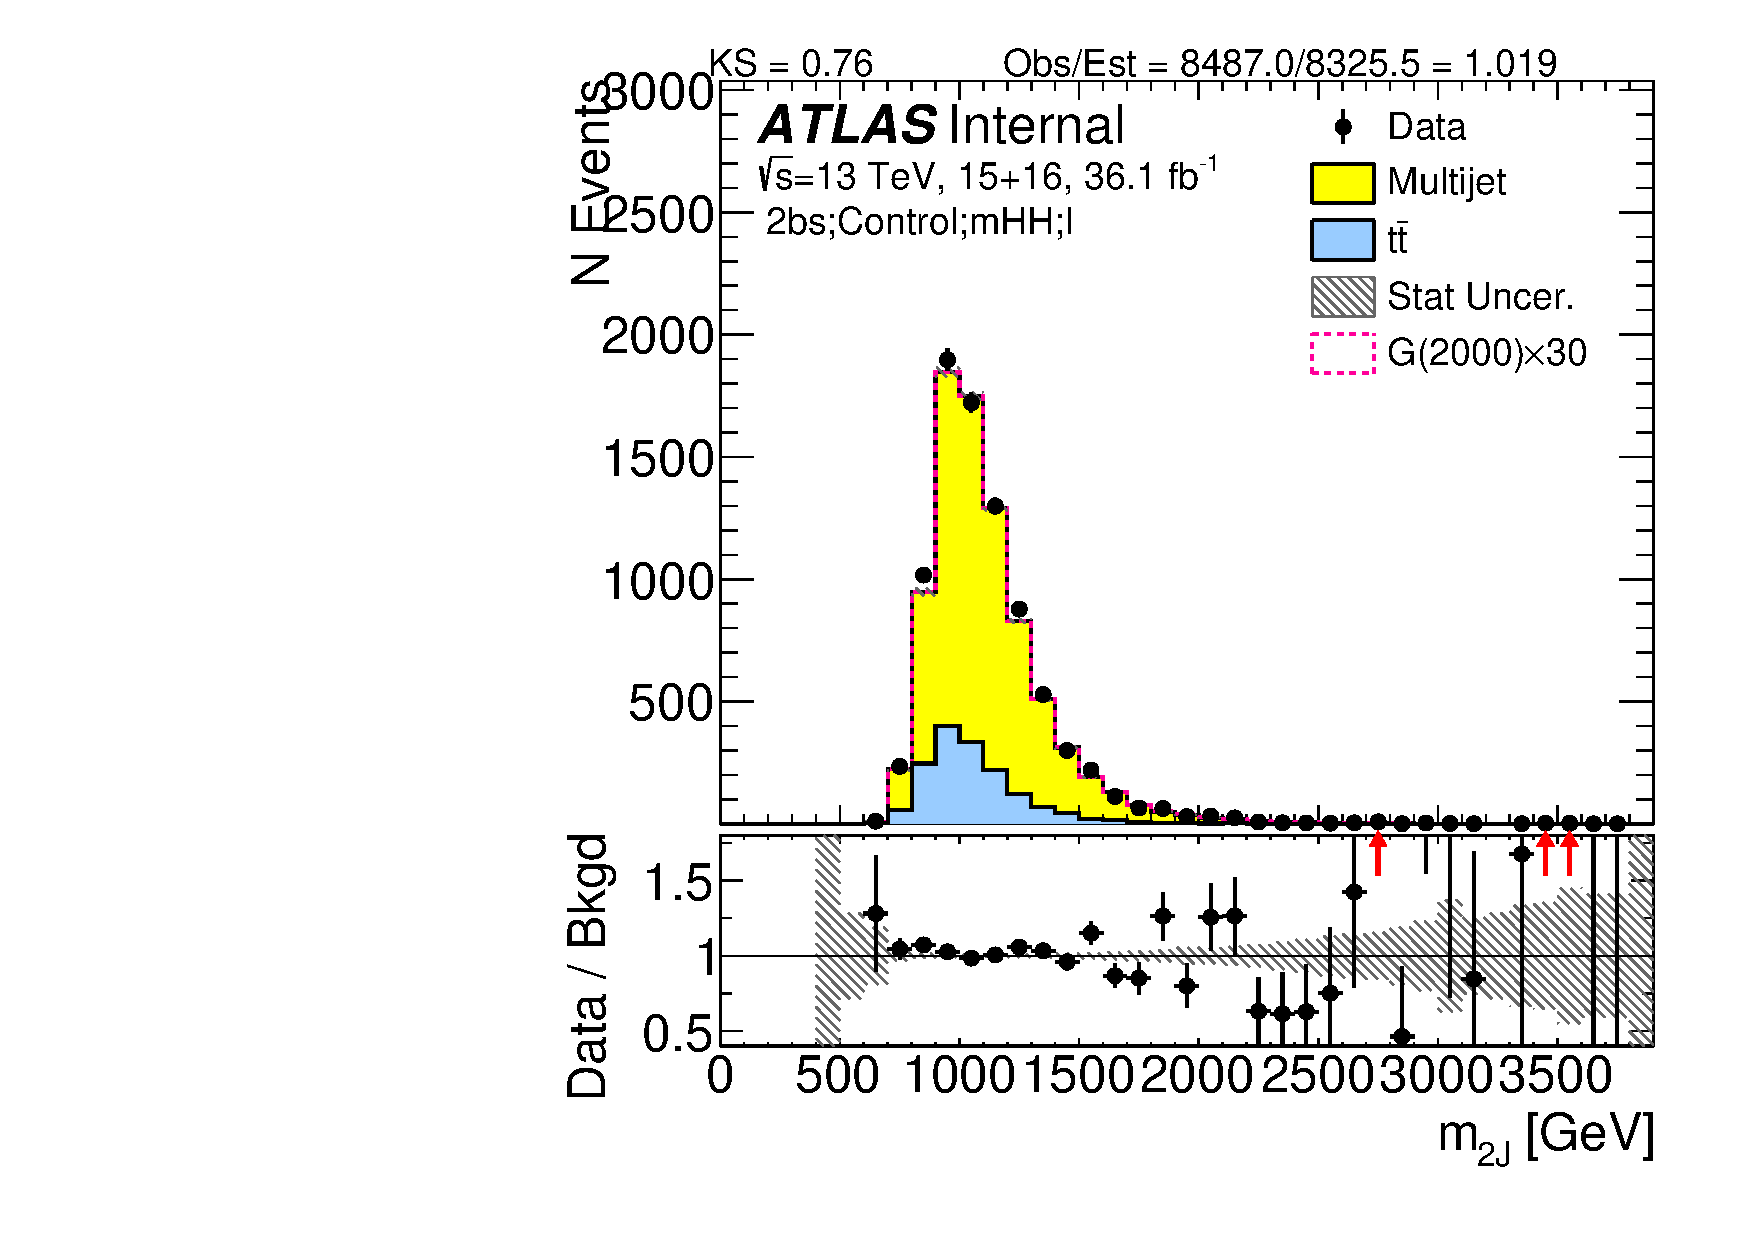
\includegraphics[angle=270, width=0.3\textwidth]{./figures/boosted/AppendixResveto/Moriond_TwoTag_split_Control_mHH_l.pdf}
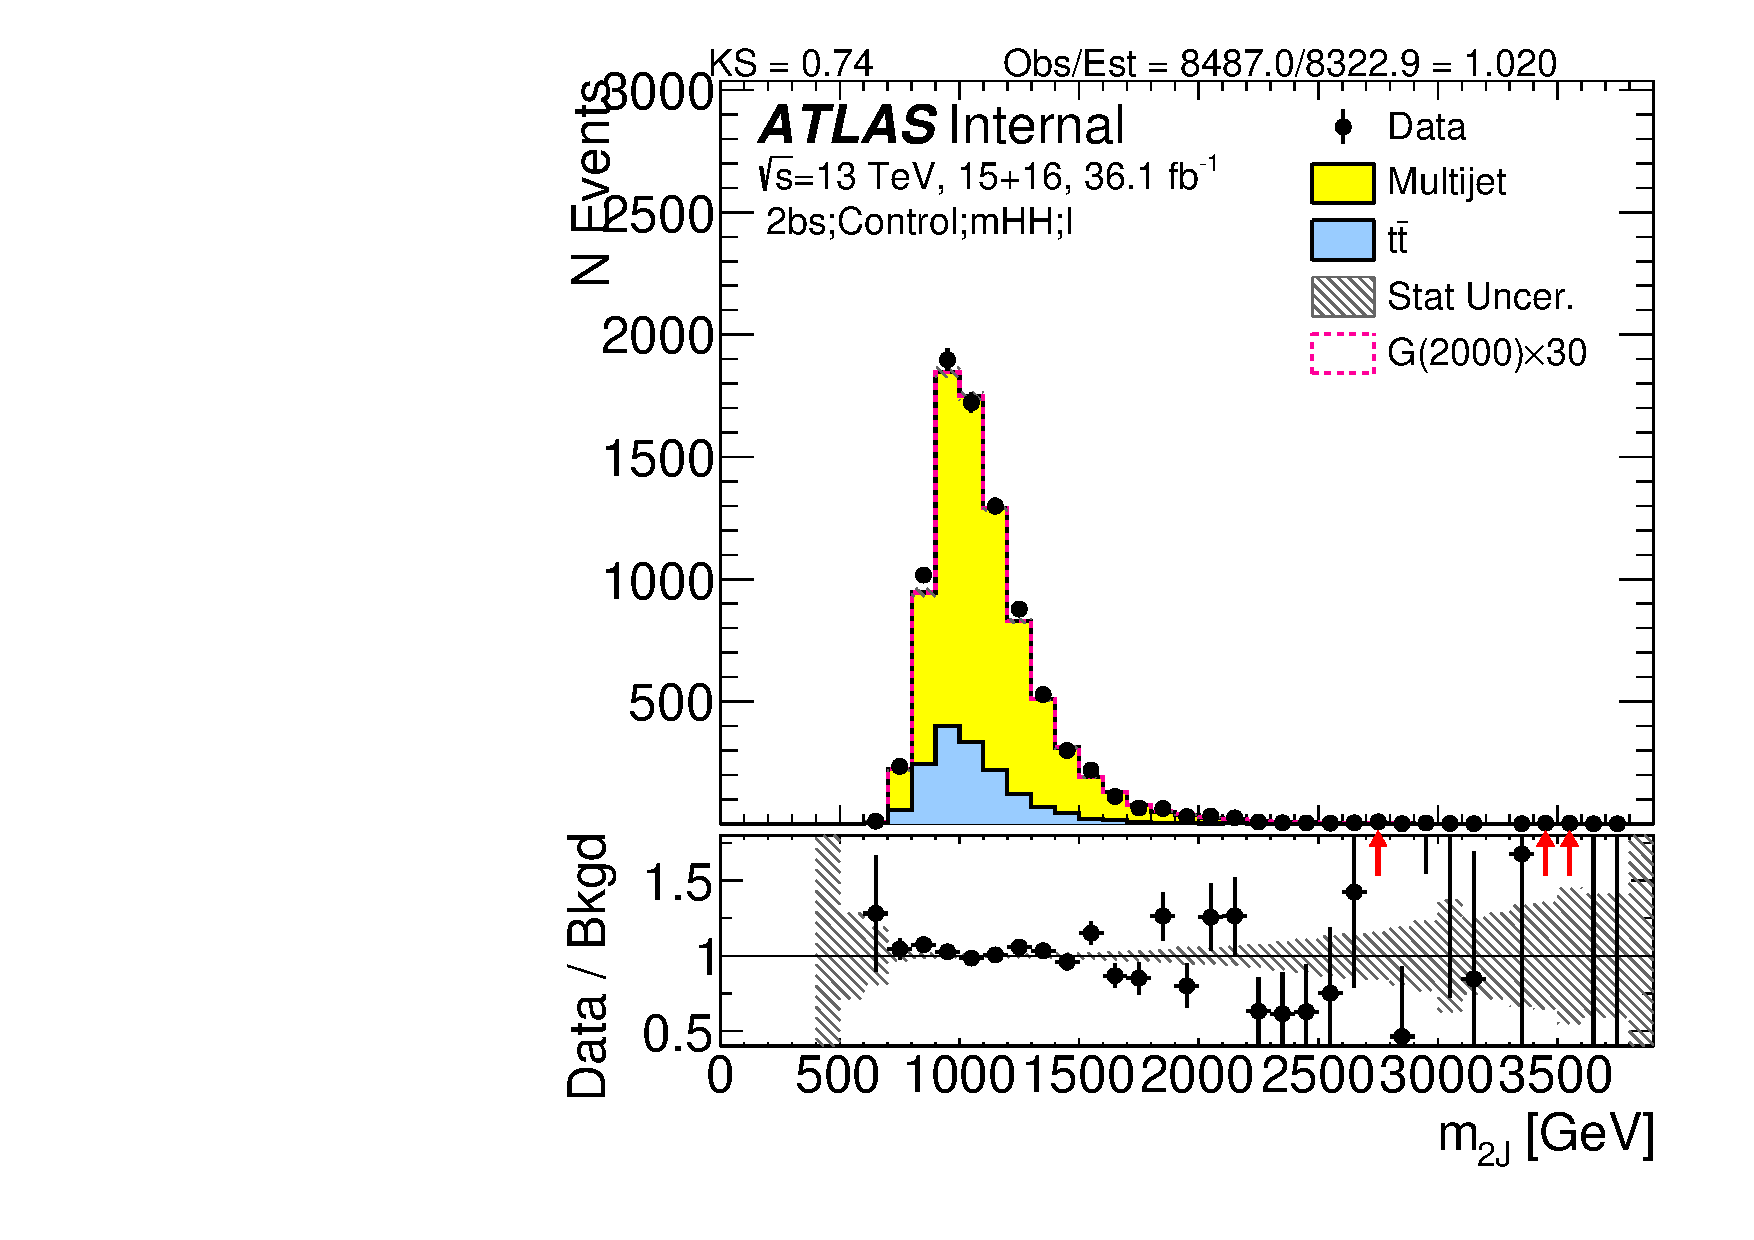
\includegraphics[angle=270, width=0.3\textwidth]{./figures/boosted/AppendixResveto/Moriond_resveto_TwoTag_split_Control_mHH_l.pdf}
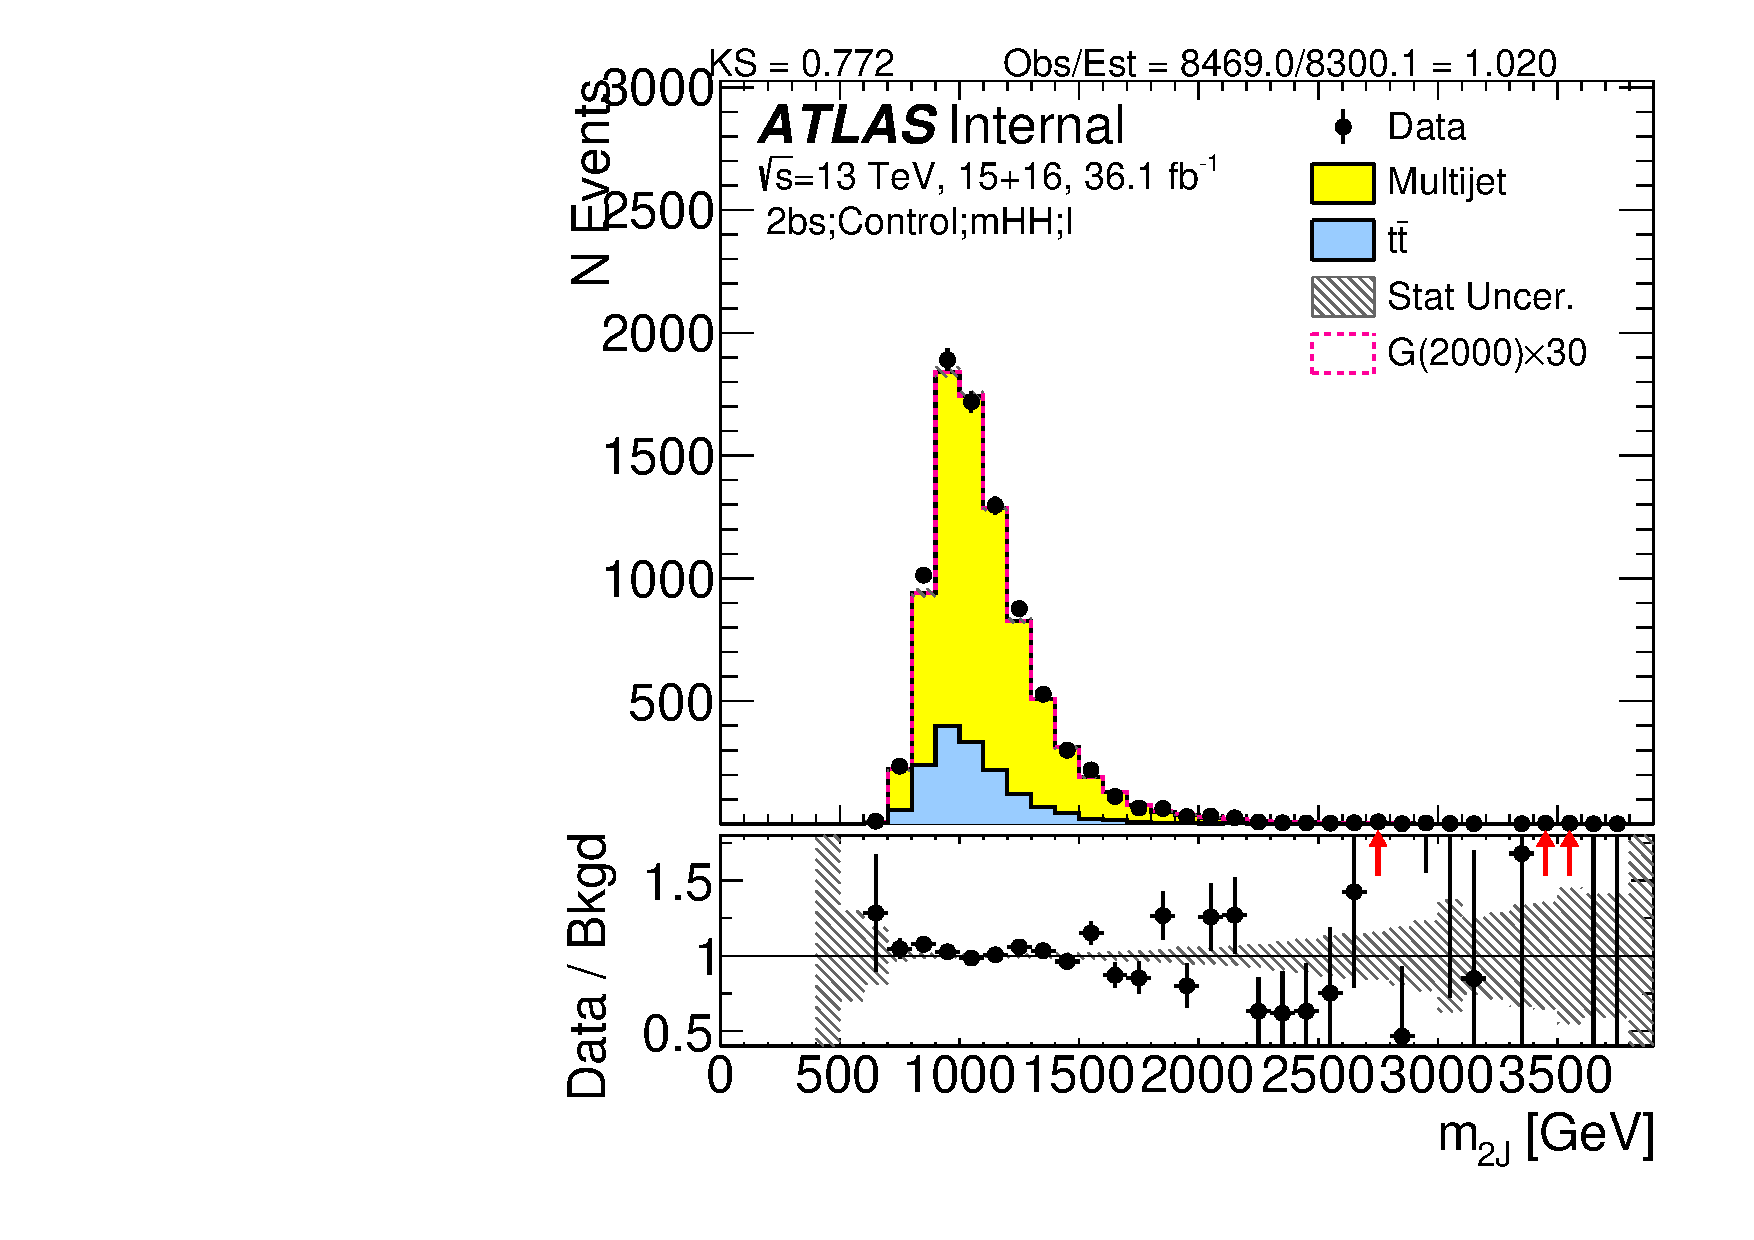
\includegraphics[angle=270, width=0.3\textwidth]{./figures/boosted/AppendixResveto/Moriond_fullresveto_TwoTag_split_Control_mHH_l.pdf}\\
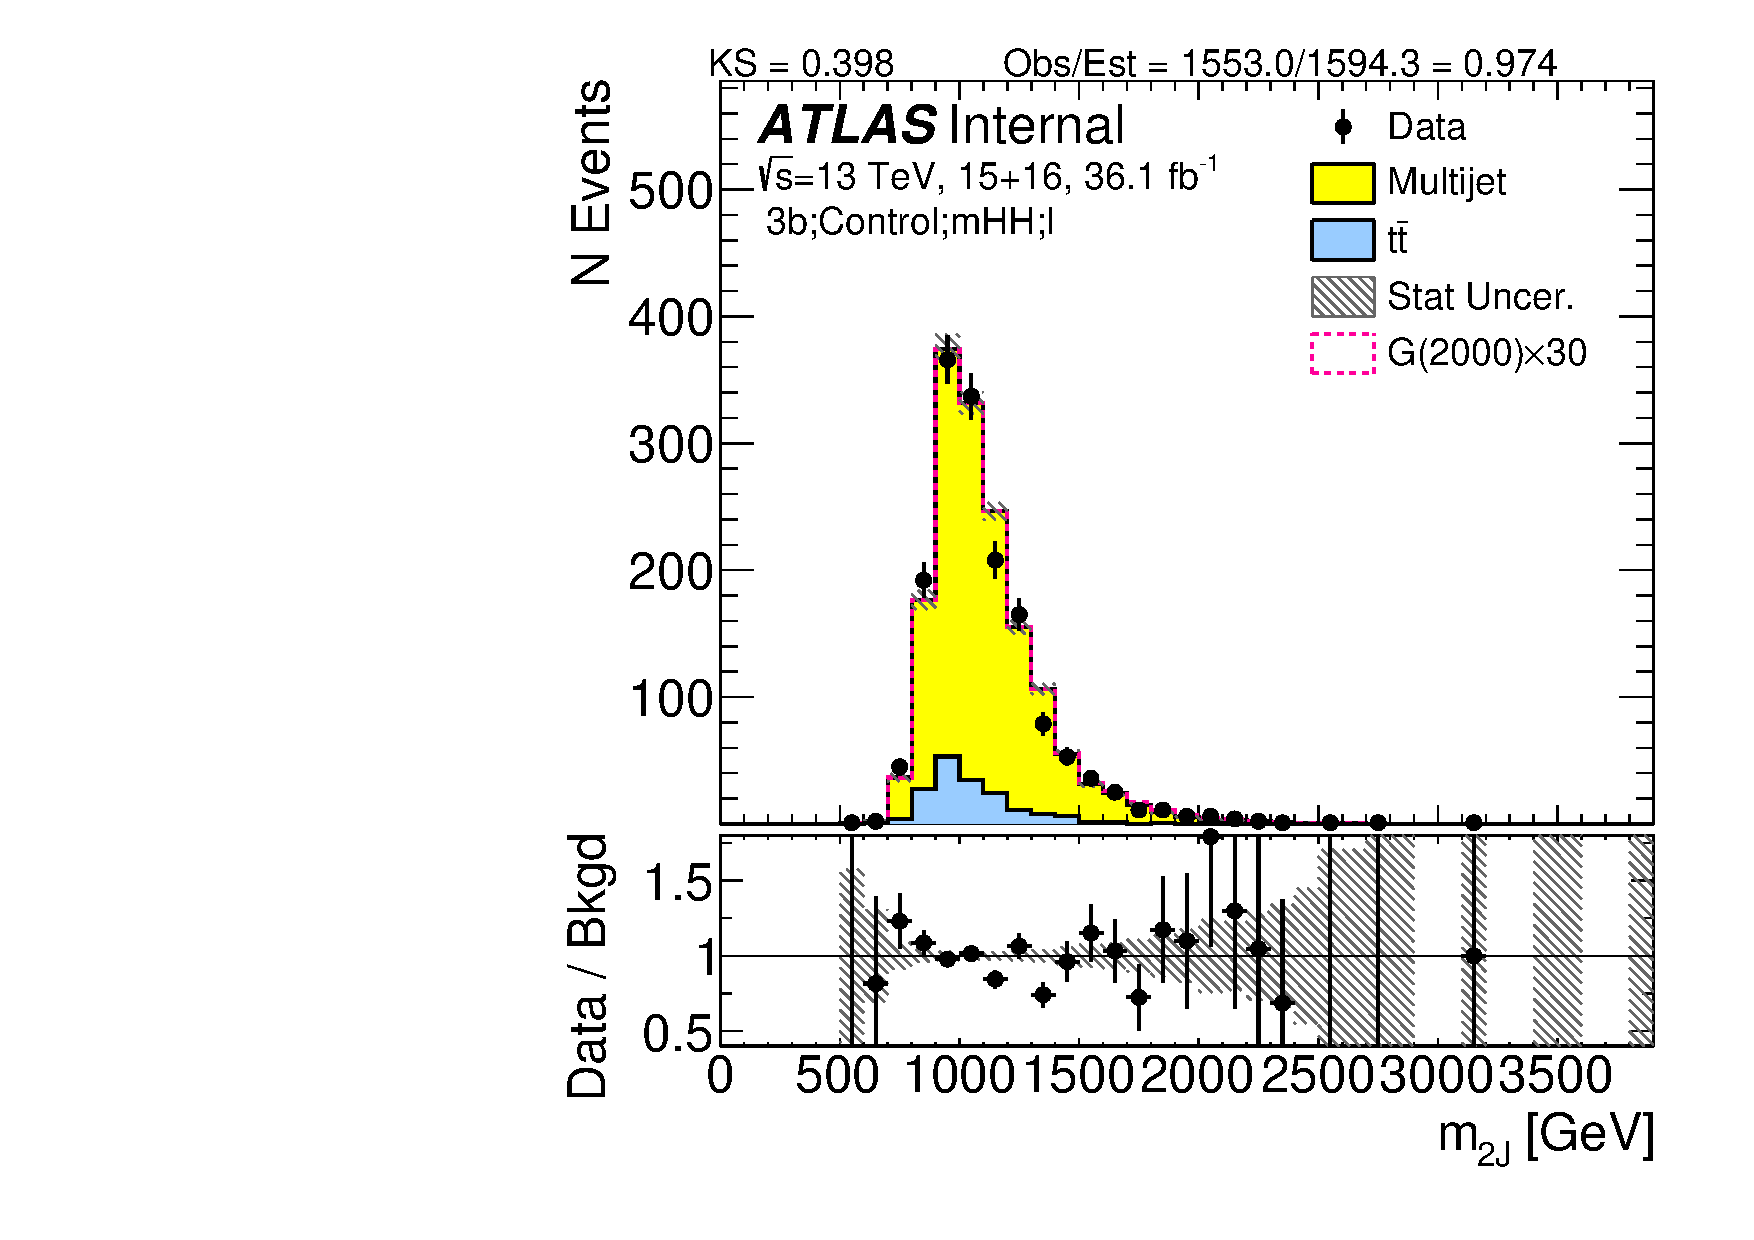
\includegraphics[angle=270, width=0.3\textwidth]{./figures/boosted/AppendixResveto/Moriond_ThreeTag_Control_mHH_l.pdf}
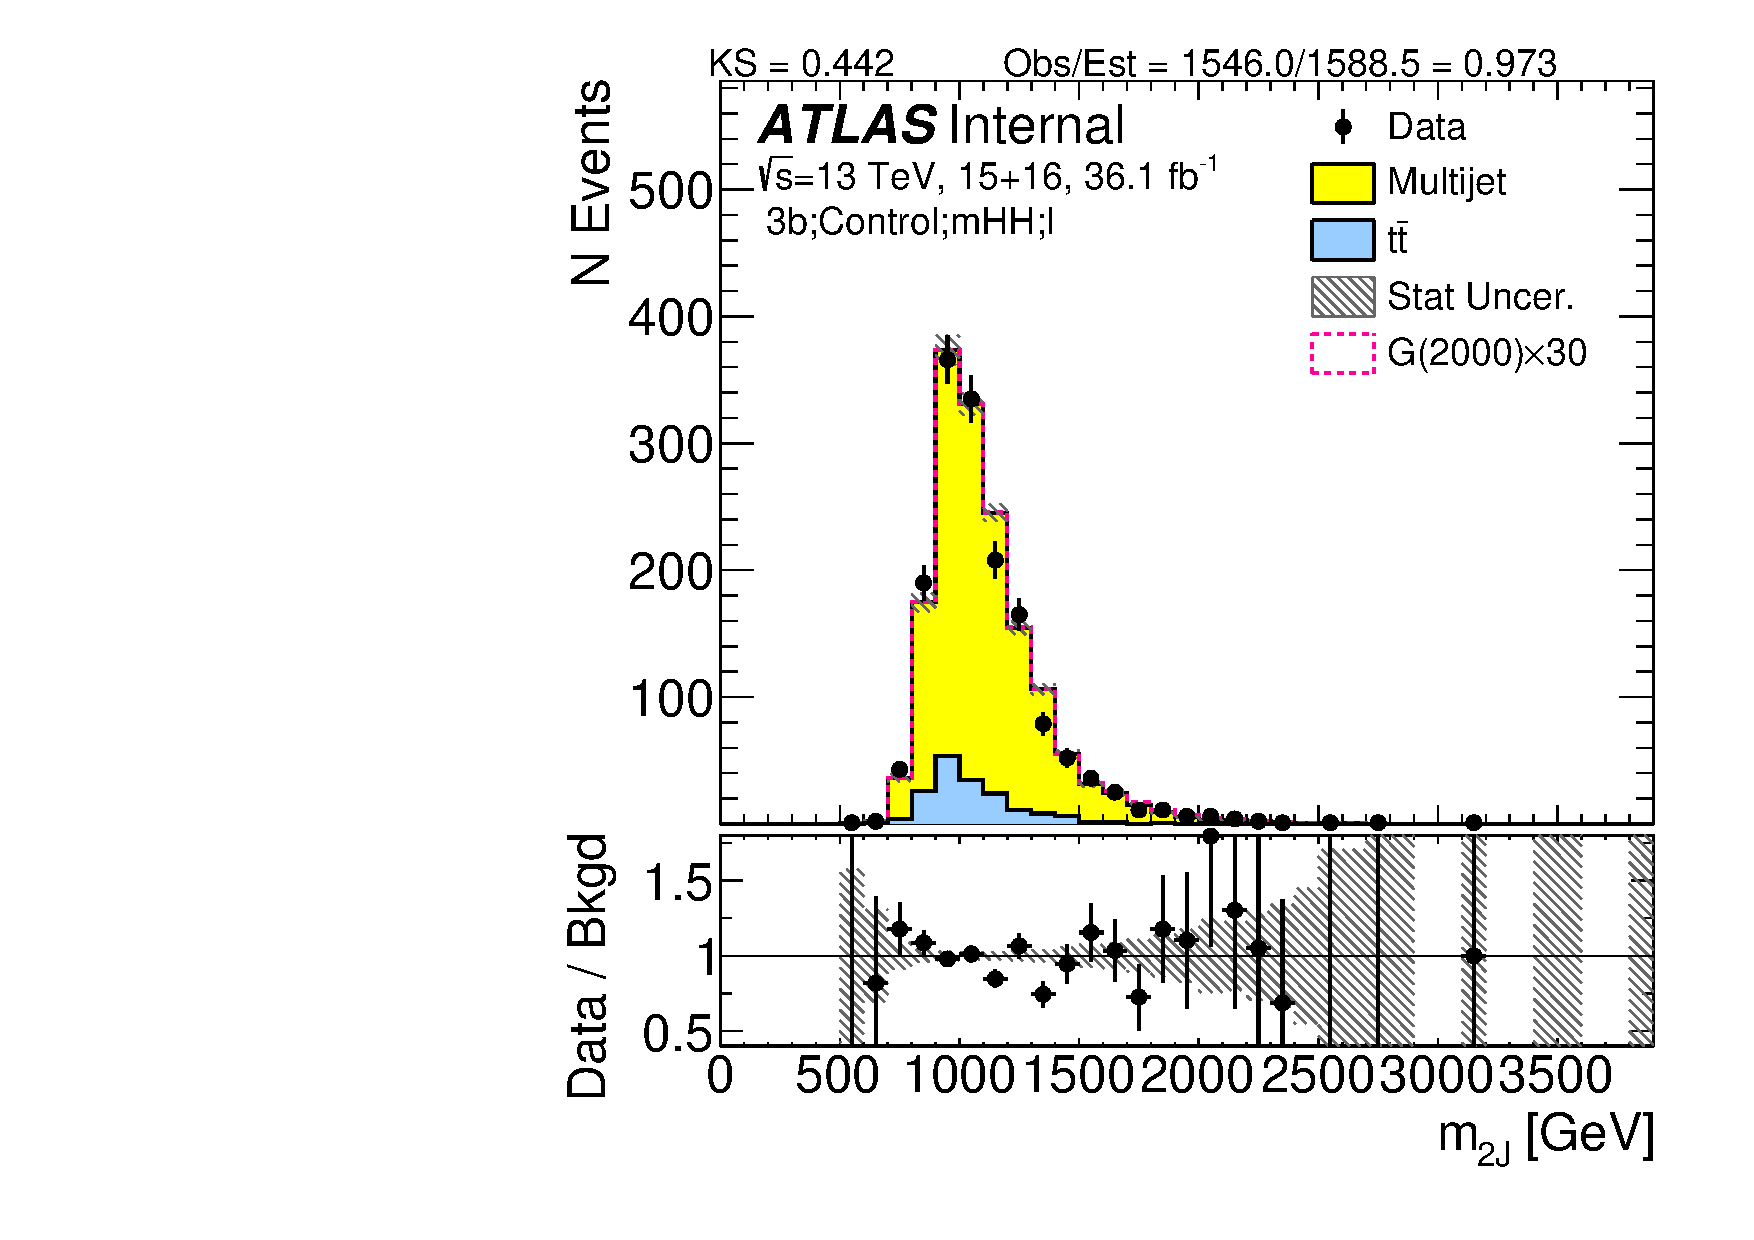
\includegraphics[angle=270, width=0.3\textwidth]{./figures/boosted/AppendixResveto/Moriond_resveto_ThreeTag_Control_mHH_l.pdf}
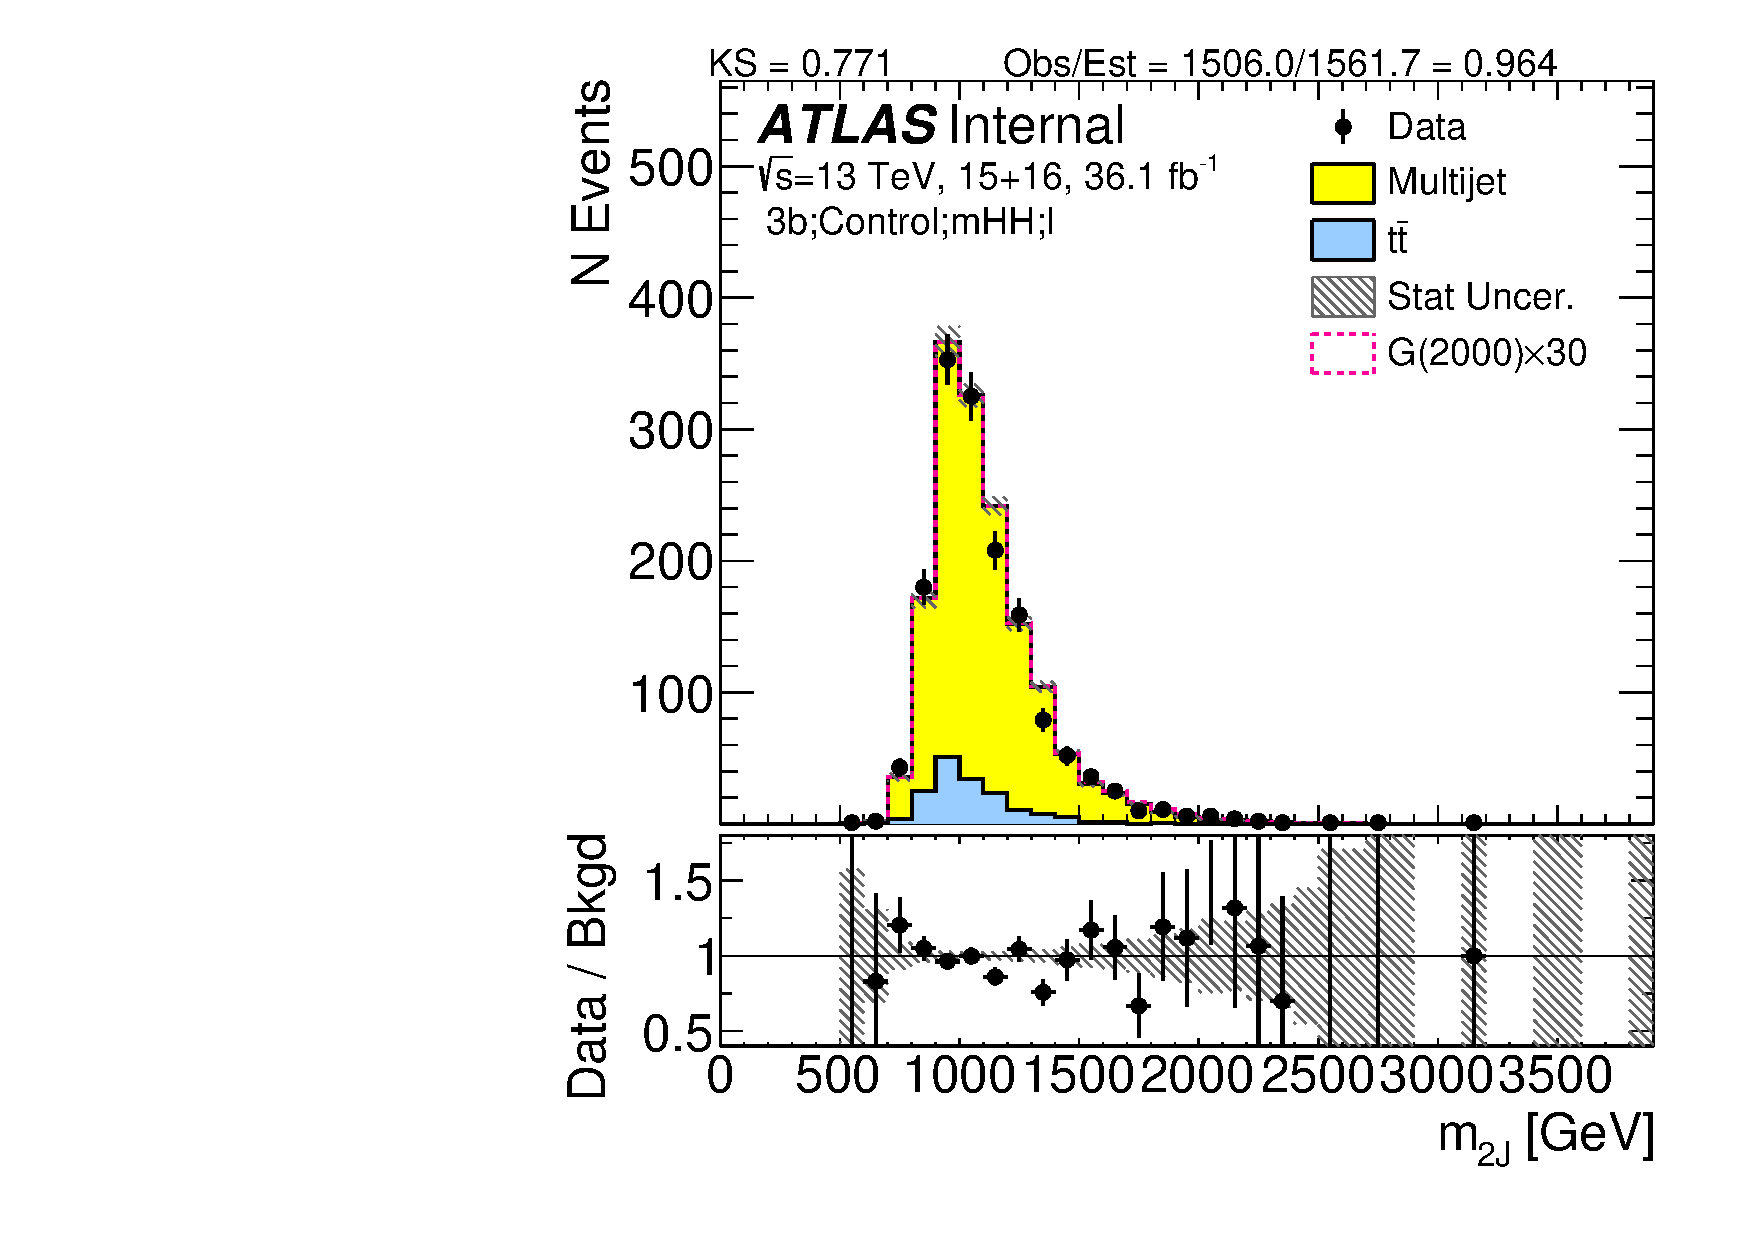
\includegraphics[angle=270, width=0.3\textwidth]{./figures/boosted/AppendixResveto/Moriond_fullresveto_ThreeTag_Control_mHH_l.pdf}\\
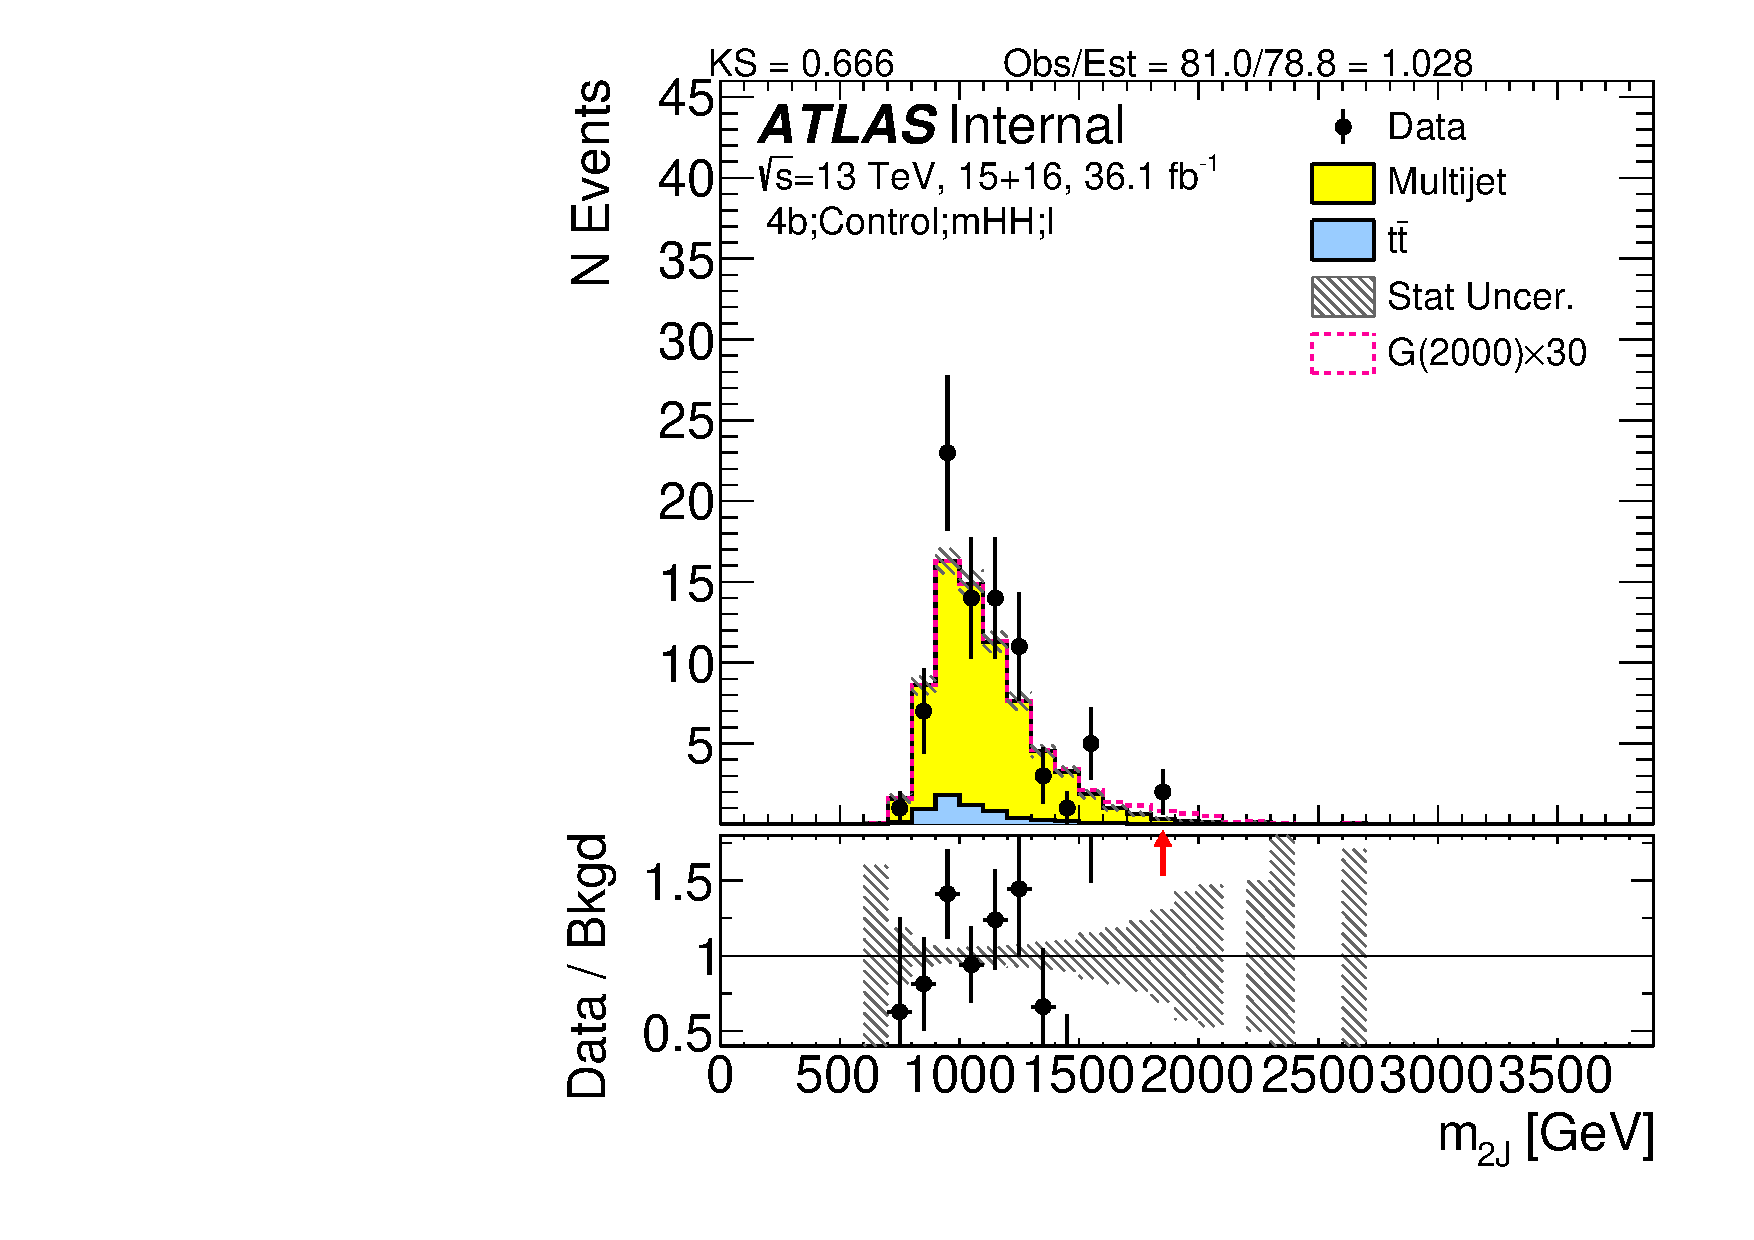
\includegraphics[angle=270, width=0.3\textwidth]{./figures/boosted/AppendixResveto/Moriond_FourTag_Control_mHH_l.pdf}
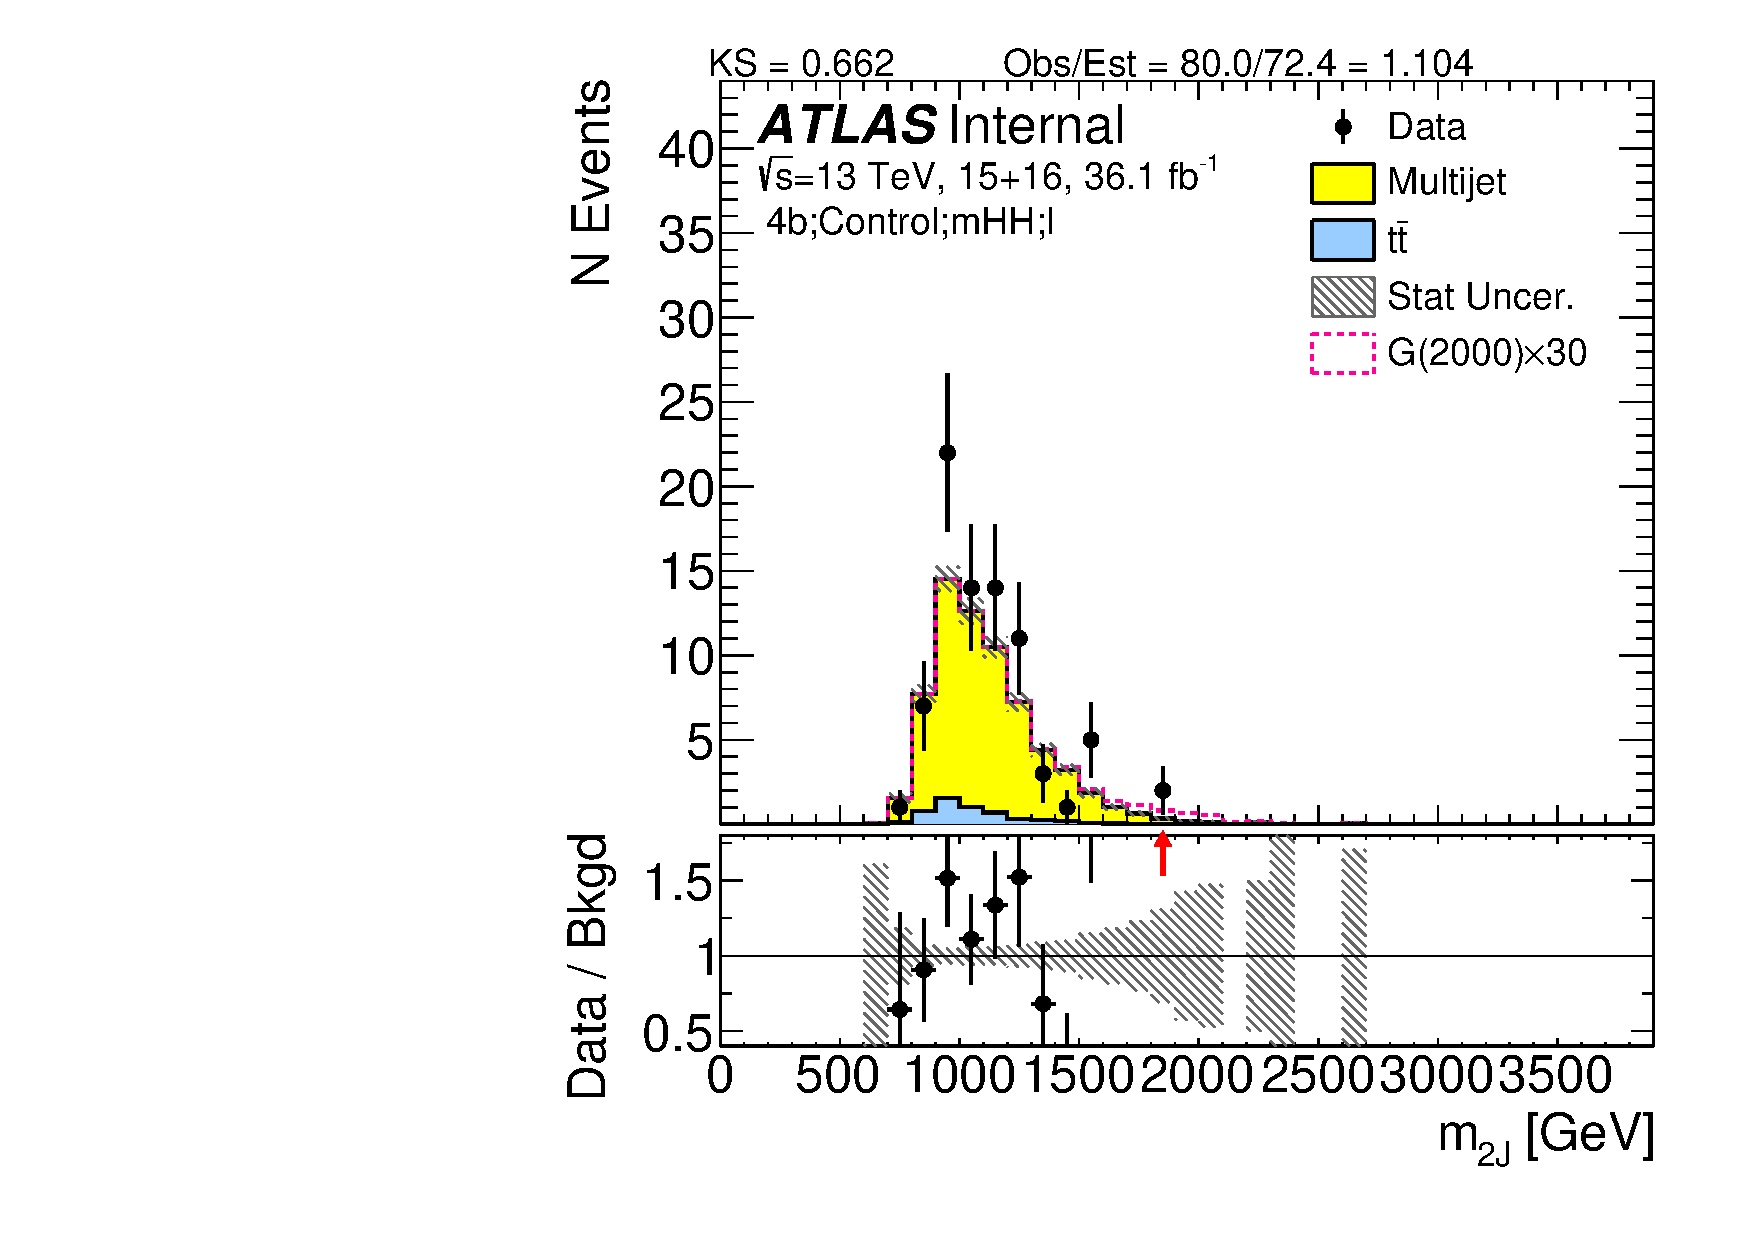
\includegraphics[angle=270, width=0.3\textwidth]{./figures/boosted/AppendixResveto/Moriond_resveto_FourTag_Control_mHH_l.pdf}
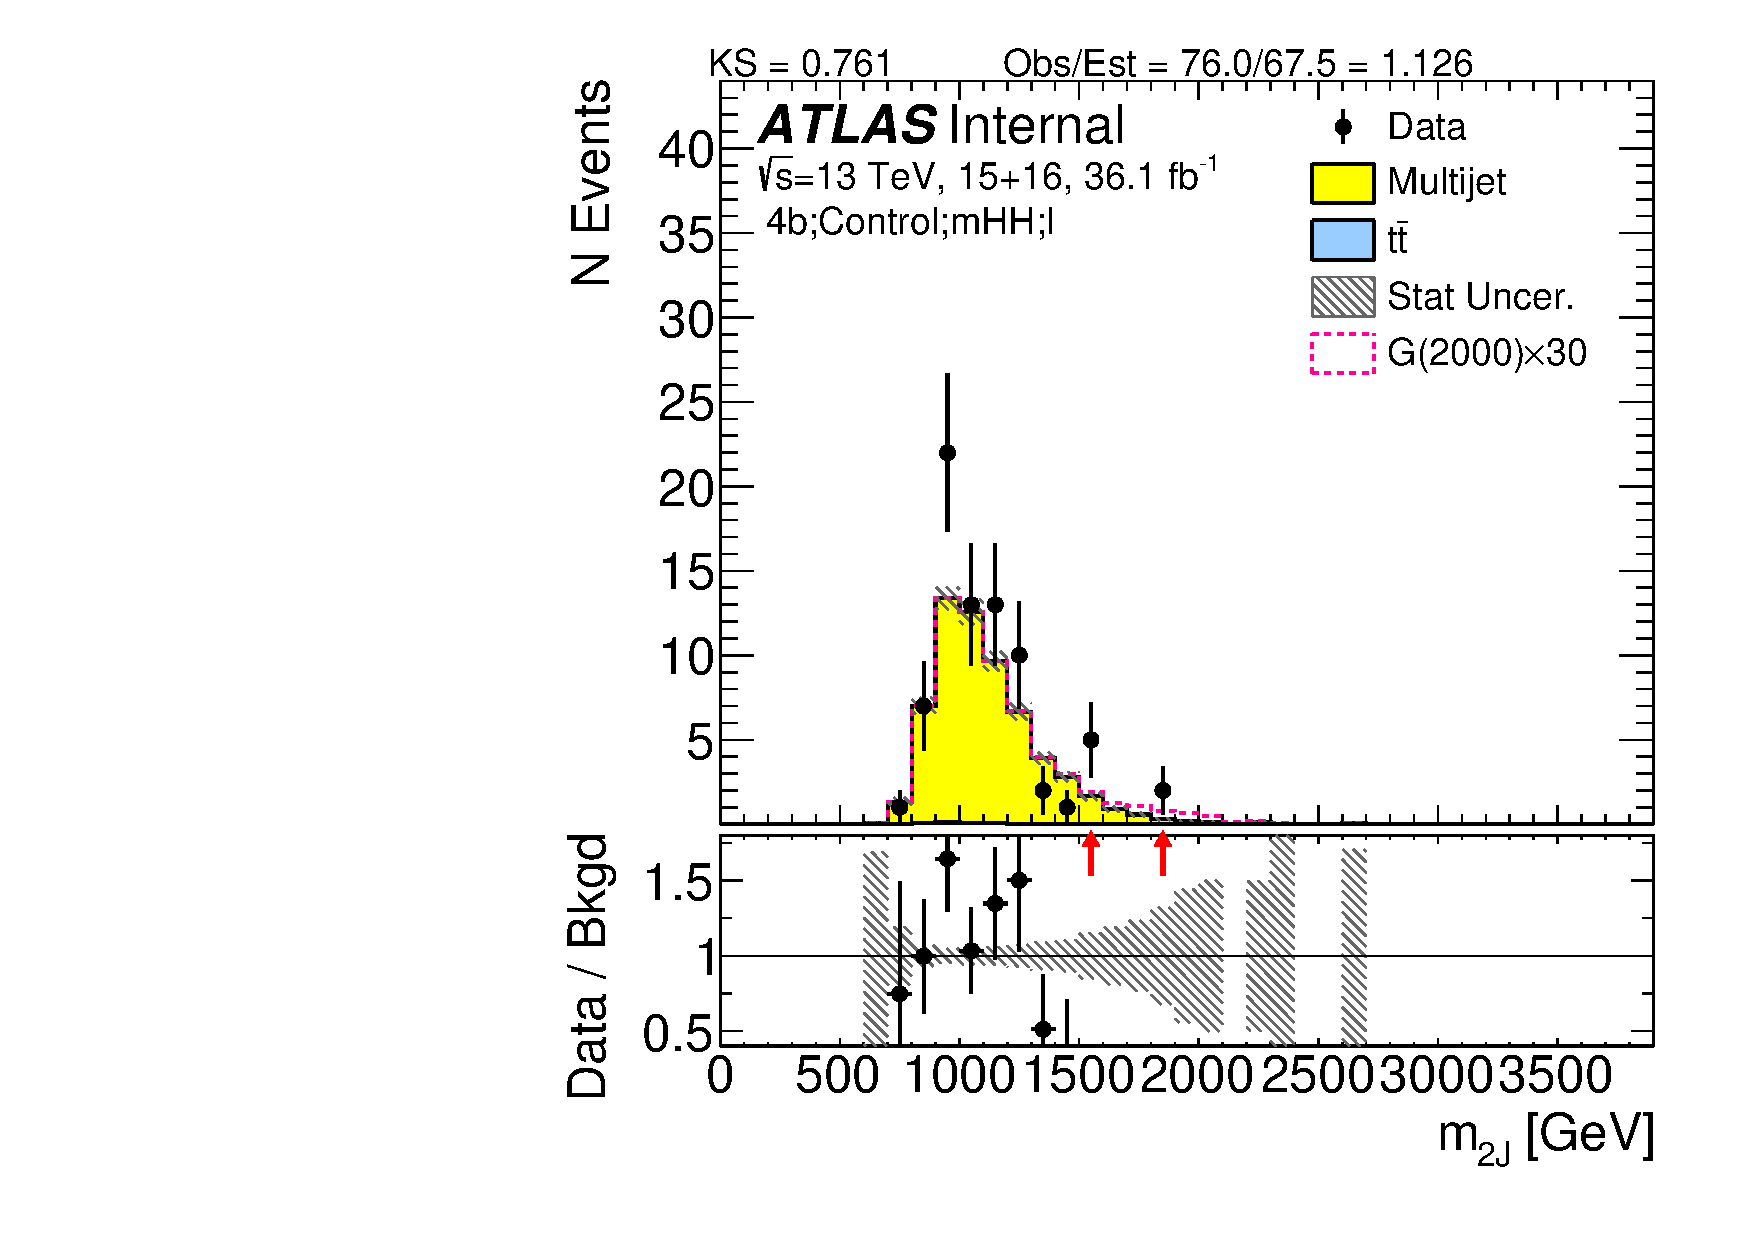
\includegraphics[angle=270, width=0.3\textwidth]{./figures/boosted/AppendixResveto/Moriond_fullresveto_FourTag_Control_mHH_l.pdf}\\
  \caption{ $M_{JJ}$ distribution in Control region for 2$b$s(top), 3$b$ (middle) and 4$b$ (bottom). The left column is with the stanard resovled veto; the middle column is with the loose resolved Signal Region, $Xhh < 3.2$ veto; the right column is with the full resolved veto.}
\label{fig:app-resveto-cr}
\end{center}
\end{figure*}


